%%------------------------------------------------------------------------------
%%Präambel
%%------------------------------------------------------------------------------
%%Klasse
%%------------------------------------------------------------------------------
\documentclass[a5paper,landscape,DIV=calc,11pt,notitlepage]{scrartcl}
%%------------------------------------------------------------------------------
%%Packages
%%------------------------------------------------------------------------------
\usepackage[headsepline=no, footsepline=no]{scrlayer-scrpage}
\usepackage[T1]{fontenc}
\usepackage{libertinus}
\usepackage[ngerman]{babel} 
\usepackage[right=24pt,left=24pt, top=24pt, bottom=24pt,twoside=false]{geometry}
\usepackage{tabularx}
\usepackage[svgnames,RGB,table]{xcolor}
\usepackage{microtype}
\usepackage[german]{layout}
\usepackage{tcolorbox}
\usepackage{hyperref}
\hypersetup{colorlinks, citecolor=, linkcolor=, urlcolor=blue,pdfauthor={Sascha Christmann},pdftitle={G\={o}j\={u}-Ry\={u} Karate-D\={o} Reusrath - Prüfungsordnung - Auszug},pdfsubject={G\={o}j\={u}-Ry\={u} Karate-D\={o}},pdfproducer={MiKTeX},pdfcreator={pdflatex}}
\usepackage{enumitem}
\usepackage{tabto}
\usepackage{amssymb}
\usepackage{amsmath}
\usepackage{mathtools}
\usepackage{booktabs}
\usepackage{multirow}
\usepackage{soul}
%%------------------------------------------------------------------------------
%%Vereinbarungen & Makros
%%------------------------------------------------------------------------------
\clearpairofpagestyles
%%------------------------------------------------------------------------------
\definecolor{YBELT}{rgb}{1,1,0.2}
\definecolor{OBELT}{rgb}{1,0.404,0}
\definecolor{GBELT}{rgb}{0.431,0.686,0.282}
\definecolor{BLBELT}{rgb}{0,0.408,1}
\definecolor{BRBELT}{rgb}{0.376,0.22,0.075}
\definecolor{GKD}{rgb}{0.53,0.086,0.102}
\newcommand{\bull}{\,\textbullet\,}
\setuldepth{a}
%%------------------------------------------------------------------------------
\tcbset{width=\textwidth,height=\textheight,right=12pt,left=12pt,colback=white,fonttitle=\bfseries,adjust text=Äpgjy}
%%------------------------------------------------------------------------------
%%Ende Präambel
%%------------------------------------------------------------------------------
\begin{document}
%%------------------------------------------------------------------------------
%%Karte_Gelb
%%------------------------------------------------------------------------------
\begin{tcolorbox}[colback=white,colframe=YBELT,coltitle=black,title=8. Kyu: Gelb]
	\renewcommand{\labelenumi}{\alph{enumi}.)}
	\renewcommand{\labelenumii}{\arabic*.}
	{\scriptsize\textbf{\textit{Der 8.\,Kyu wird in aller Regel gemeinsam mit dem 9.\,Kyu absolviert, daher ist für diese Prüfung die doppelte Prüfungsgebühr, für entsprechend 2 Prüfungsmarken, zu entrichten.}}\newline Anmerkung zum (\textit{Chisai-no-})Mawashi-Geri: in der Chisai-Form wird diese Technik als kleiner Halbkreisfußtritt ohne Drehung des Standbeins ausgeführt und ist technisch vollkommen ausreichend. Die sportliche Variante kann und darf aber auch trainiert und gezeigt werden.\newline
	\begin{tabularx}{\textwidth}{lX}
		\textit{Vorausgesetzte Techniken}:& Zuki, Age-Uke, Yoko-Uke, Harai-Otoshi-Uke, Soto-Uke, Mae-Geri, \textit{(Chisai-no-)}Mawashi-Geri
	\end{tabularx}\\}\vspace{12pt}
	\begin{enumerate}[nosep]
		\item \textit{\textbf{Kihon-Ido}}:
		\begin{enumerate}[nosep]
			\item Harai-Otoshi-Uke\bull Gyaku-Zuki Ch\={u}dan\tabto{280pt}(Zenkutsu-Dachi)
			\item Mae-Geri Ch\={u}dan\tabto{280pt}(Zenkutsu-Dachi)
			\item \textit{(Chisai-no-)}Mawashi-Geri Ch\={u}dan\tabto{280pt}(Zenkutsu-Dachi)
			\item Oi-Zuki J\={o}dan\bull Gyaku-Zuki Ch\={u}dan\tabto{280pt}(Zenkutsu-Dachi)
			\item Soto-Uke Ch\={u}dan\bull Gyaku-Zuki Ch\={u}dan\tabto{280pt}(Zenkutsu-Dachi)
			\item Age-Uke\bull Gyaku-Zuki J\={o}dan\tabto{280pt}(Sanchin-Dachi)
			\item Yoko-Uke\bull Gyaku-Zuki Ch\={u}dan\tabto{280pt}(Sanchin-Dachi)
		\end{enumerate}\vspace{24pt}
		\item \textit{\textbf{Kata}}:
		\begin{enumerate}[nosep]
			\item Taikyoku J\={o}dan
			\item Taikyoku Ch\={u}dan
		\end{enumerate}\vspace{24pt}
		\item \textit{\textbf{Partnerformen}}:
		\begin{enumerate}[nosep]
			\item Kihon-Ippon Kumite\tabto{280pt}J\={o}dan\bull Ch\={u}dan (ggf. Gedan)
		\end{enumerate}
	\end{enumerate}
\end{tcolorbox}
%%------------------------------------------------------------------------------
\pagebreak
%%------------------------------------------------------------------------------
%%Karte_Orange
%%------------------------------------------------------------------------------
\begin{tcolorbox}[colback=white,colframe=OBELT,coltitle=white,title=7. Kyu: Orange]
	\renewcommand{\labelenumi}{\alph{enumi}.)}
	\renewcommand{\labelenumii}{\arabic*.}
	{\scriptsize
		\begin{tabularx}{\textwidth}{lX}
			\textit{Vorausgesetzte Techniken}:& Zuki, Age-Uke, Yoko-Uke, Harai-Otoshi-Uke, Soto-Uke, Uraken-Uchi, Empi-Age-Uchi, Mae-Geri, \mbox{\textit{(Chisai-no-)}Mawashi-Geri}
		\end{tabularx}\\}\vspace{12pt}
	\begin{enumerate}[nosep]
		\item \textit{\textbf{Kihon-Ido}}:
		\begin{enumerate}[nosep]
			\item Harai-Otoshi-Uke\bull Gyaku-Zuki Ch\={u}dan\tabto{280pt}(Zenkutsu-Dachi)
			\item Oi-Zuki J\={o}dan\bull Gyaku-Zuki Ch\={u}dan\tabto{280pt}(Zenkutsu-Dachi)
			\item Soto-Uke Ch\={u}dan\bull Gyaku-Zuki Ch\={u}dan\tabto{280pt}(Zenkutsu-Dachi)
			\item Kansetsu-Geri Gedan\tabto{280pt}(Sanchin-Dachi)
			\item Age-Uke\bull Gyaku-Zuki J\={o}dan\tabto{280pt}(Sanchin-Dachi)
			\item Yoko-Uke\bull Gyaku-Zuki Ch\={u}dan\tabto{280pt}(Sanchin-Dachi)
			\item Harai-Otoshi-Uke\bull Gyaku-Zuki Ch\={u}dan\tabto{280pt}(Shiko-Dachi 45°)
		\end{enumerate}\vspace{24pt}
		\item \textit{\textbf{Kata}}:
		\begin{enumerate}[nosep]
			\item Taikyoku (welche Taikyoku geprüft wird, entscheidet der Prüfer)
			\item Gekisai-Dai-Ichi
		\end{enumerate}\vspace{24pt}
		\item \textit{\textbf{Partnerformen}}:
		\begin{enumerate}[nosep]
			\item Kihon-Ippon Kumite\tabto{280pt}J\={o}dan\bull Ch\={u}dan (ggf. Gedan)
		\end{enumerate}
	\end{enumerate}
\end{tcolorbox}
%%------------------------------------------------------------------------------
\pagebreak
%%------------------------------------------------------------------------------
%%Karte_Grün
%%------------------------------------------------------------------------------
\begin{tcolorbox}[colback=white,colframe=GBELT,coltitle=white,title=6. Kyu: Grün]
	\renewcommand{\labelenumi}{\alph{enumi}.)}
	\renewcommand{\labelenumii}{\arabic*.}
	{\scriptsize
		\begin{tabularx}{\textwidth}{lX}
			\textit{Vorausgesetzte Techniken}:& Zuki, Age-Uke, Yoko-Uke, Harai-Otoshi-Uke, Soto-Uke,Kake-Uke, Mawashi-Uke, Uraken-Uchi, Empi-Age-Uchi, Mae-Geri, \textit{(Chisai-no-)}Mawashi-Geri, Kansetsu-Geri
		\end{tabularx}\\}\vspace{12pt}
	\begin{enumerate}[nosep]
		\item \textit{\textbf{Kihon-Ido}}:
		\begin{enumerate}[nosep]
			\item Harai-Otoshi-Uke\bull Mae-Geri Ch\={u}dan\bull Gyaku-Zuki Ch\={u}dan\tabto{280pt}(Zenkutsu-Dachi)
			\item \textit{(Chisai-no-)}Mawashi-Geri Ch\={u}dan\bull Gyaku-Zuki Ch\={u}dan\tabto{280pt}(Zenkutsu-Dachi)
			\item Age-Uke\bull Gyaku-Zuki Ch\={u}dan\bull Mae-Geri Ch\={u}dan\tabto{280pt}(Zenkutsu-Dachi)
			\item Yoko-Uke\bull Ren-Zuki J\={o}dan-Ch\={u}dan\tabto{280pt}(Sanchin-Dachi)
			\item Harai-Otoshi-Uke\bull Gyaku-Zuki Ch\={u}dan\tabto{280pt}(Shiko-Dachi 45°)
			\item Kake-Uke\bull Mae-Geri Ch\={u}dan\tabto{280pt}(Neko-Ashi-Dachi)
		\end{enumerate}\vspace{24pt}
		\item \textit{\textbf{Kata}}:
		\begin{enumerate}[nosep]
			\item Gekisai-Dai-Ichi
			\item Gekisai-Dai-Ni
		\end{enumerate}\vspace{24pt}
		\item \textit{\textbf{Partnerformen (2 aus 3)}}:
		\begin{enumerate}[nosep]
			\item Yakusoku-Kumite\tabto{200pt}3 Kumite-Ura\bull 3 Nage-Waza (frei auszuwählen)
			\item Shiai-Kumite\tabto{200pt}Jiyu-Kumite 1 Minute \frqq Freikampf\flqq~(sportlich)
			\item Alternativ zum Shiai-Kumite\tabto{200pt}SV
		\end{enumerate}
	\end{enumerate}
\end{tcolorbox}
%%------------------------------------------------------------------------------
\pagebreak
%%------------------------------------------------------------------------------
%%Karte_Blau_1
%%------------------------------------------------------------------------------
\begin{tcolorbox}[colback=white,colframe=BLBELT,coltitle=white,title=5. Kyu: Blau]
	\renewcommand{\labelenumi}{\alph{enumi}.)}
	\renewcommand{\labelenumii}{\arabic*.}
	{\scriptsize
		\begin{tabularx}{\textwidth}{lX}
			\textit{Vorausgesetzte Techniken}:& Zuki, Age-Uke, Yoko-Uke, Harai-Otoshi-Uke, Soto-Uke, Kake-Uke, Mawashi-Uke, Teish\={o}-Uchi, Uraken-Uchi, \mbox{Empi-Age-Uchi}, Mae-Geri, \textit{(Chisai-no-)}Mawashi-Geri, Kansetsu-Geri
		\end{tabularx}\\}\vspace{12pt}
	\begin{enumerate}[nosep]
		\item \textit{\textbf{Kihon-Ido}}:
		\begin{enumerate}[nosep]
			\item Harai-Otoshi-Uke\bull Mae-Geri Ch\={u}dan\bull Gyaku-Zuki Ch\={u}dan\tabto{280pt}(Zenkutsu-Dachi)
			\item \textit{(Chisai-no-)}Mawashi-Geri Ch\={u}dan\bull Gyaku-Zuki Ch\={u}dan\tabto{280pt}(Zenkutsu-Dachi)
			\item Age-Uke\bull Gyaku-Zuki Ch\={u}dan\bull Mae-Geri Ch\={u}dan\tabto{280pt}(Zenkutsu-Dachi)
			\item Yoko-Uke\bull Ren-Zuki J\={o}dan-Ch\={u}dan\tabto{280pt}(Sanchin-Dachi)
			\item Harai-Otoshi-Uke\bull Gyaku-Zuki Ch\={u}dan\tabto{280pt}(Shiko-Dachi 45°)
			\item Kake-Uke\bull Mae-Geri Ch\={u}dan\tabto{280pt}(Neko-Ashi-Dachi)
		\end{enumerate}\vspace{24pt}
		\item \textit{\textbf{Kata}}:
		\begin{enumerate}[nosep]
			\item Gekisai-Dai-Ni
			\item Saif\={a}
		\end{enumerate}\vspace{24pt}
		\item \textit{\textbf{Partnerformen (2 aus 3)}}:
		\begin{enumerate}[nosep]
			\item Yakusoku-Kumite\tabto{200pt}3 Kumite-Ura\bull 3 Nage-Waza (frei auszuwählen)
			\item Shiai-Kumite\tabto{200pt}Jiyu-Kumite 1 Minute \frqq Freikampf\flqq~(sportlich)
			\item Alternativ zum Shiai-Kumite\tabto{200pt}SV
		\end{enumerate}
	\end{enumerate}
\end{tcolorbox}
%%------------------------------------------------------------------------------
\pagebreak
%%------------------------------------------------------------------------------
%%Karte_Blau_2
%%------------------------------------------------------------------------------
\begin{tcolorbox}[colback=white,colframe=BLBELT,coltitle=white,title=4. Kyu: Blau]
	\renewcommand{\labelenumi}{\alph{enumi}.)}
	\renewcommand{\labelenumii}{\arabic*.}
	{\scriptsize
		\begin{tabularx}{\textwidth}{lX}
			\textit{Vorausgesetzte Techniken}:& Zuki, Age-Uke, Yoko-Uke, Harai-Otoshi-Uke, Soto-Uke, Kake-Uke, Mawashi-Uke, Teish\={o}-Uchi, Uraken-Uchi, \mbox{Empi-Age-Uchi}, Mae-Geri, \textit{(Chisai-no-)}Mawashi-Geri, Kansetsu-Geri
		\end{tabularx}\\}\vspace{12pt}
	\begin{enumerate}[nosep]
		\item \textit{\textbf{Kihon-Ido}}:
		\begin{enumerate}[nosep]
			\item Harai-Otoshi-Uke\bull Mae-Geri Ch\={u}dan\bull Gyaku-Zuki Ch\={u}dan\tabto{280pt}(Zenkutsu-Dachi)
			\item \textit{(Chisai-no-)}Mawashi-Geri Ch\={u}dan\bull Gyaku-Zuki Ch\={u}dan\tabto{280pt}(Zenkutsu-Dachi)
			\item Age-Uke\bull Gyaku-Zuki Ch\={u}dan\bull Mae-Geri Ch\={u}dan\tabto{280pt}(Zenkutsu-Dachi)
			\item Yoko-Uke\bull Ren-Zuki J\={o}dan-Ch\={u}dan\tabto{280pt}(Sanchin-Dachi)
			\item Harai-Otoshi-Uke\bull Gyaku-Zuki Ch\={u}dan\tabto{280pt}(Shiko-Dachi 45°)
			\item Kake-Uke\bull Mae-Geri Ch\={u}dan\tabto{280pt}(Neko-Ashi-Dachi)
		\end{enumerate}\vspace{24pt}
		\item \textit{\textbf{Kata}}:
		\begin{enumerate}[nosep]
			\item Saif\={a}
			\item S\={e}enchin
		\end{enumerate}\vspace{24pt}
		\item \textit{\textbf{Partnerformen (2 aus 3)}}:
		\begin{enumerate}[nosep]
			\item Yakusoku-Kumite\tabto{200pt}3 Kumite-Ura\bull 3 Nage-Waza (frei auszuwählen)
			\item Shiai-Kumite\tabto{200pt}Jiyu-Kumite 1 Minute \frqq Freikampf\flqq~(sportlich)
			\item Alternativ zum Shiai-Kumite\tabto{200pt}SV
		\end{enumerate}
	\end{enumerate}
\end{tcolorbox}
%%------------------------------------------------------------------------------
\pagebreak
%%------------------------------------------------------------------------------
%%Karte_Braun_1
%%------------------------------------------------------------------------------
\begin{tcolorbox}[colback=white,colframe=BRBELT,coltitle=white,title=3. Kyu: Braun]
	\renewcommand{\labelenumi}{\alph{enumi}.)}
	\renewcommand{\labelenumii}{\arabic*.}
	{\scriptsize 
		\begin{tabularx}{\textwidth}{lX}
			\textit{Vorausgesetzte Techniken}:& Zuki, Age-Uke, Yoko-Uke, Harai-Otoshi-Uke, Soto-Uke, Kake-Uke, Mawashi-Uke, Teish\={o}-Uchi, Uraken-Uchi, \mbox{Empi-Age-Uchi}, Mae-Geri, \textit{(Chisai-no-)}Mawashi-Geri, Kansetsu-Geri
		\end{tabularx}\\}\vspace{12pt}
	\begin{enumerate}[nosep]
		\item \textit{\textbf{Kihon-Ido}}:
		\begin{enumerate}[nosep]
			\item Harai-Otoshi-Uke\bull Mae-Geri Ch\={u}dan\bull Gyaku-Zuki Ch\={u}dan\tabto{280pt}(Zenkutsu-Dachi)
			\item Kizami-Zuki J\={o}dan\bull Gyaku-Zuki Ch\={u}dan\tabto{280pt}(Suri-Ashi/Zenkutsu-Dachi)
			\item Soto-Uke Ch\={u}dan\bull Uraken-Uchi J\={o}dan\tabto{280pt}(Sanchin-Dachi)
			\item Kake-Uke\bull Ren-Zuki J\={o}dan-Ch\={u}dan\tabto{280pt}(Sanchin-Dachi)
			\item Harai-Otoshi-Uke\bull Gyaku-Zuki Ch\={u}dan\tabto{280pt}(Shiko-Dachi 45°)
			\item Shut\={o}-Uke\bull Kansetsu-Geri Gedan\tabto{280pt}(Neko-Ashi-Dachi)
		\end{enumerate}\vspace{24pt}
		\item \textit{\textbf{Kata}}:\tabto{200pt}\textit{\textbf{Kata\,Bunkai}}:
		\begin{enumerate}[nosep]
			\item S\={e}enchin\tabto{200pt}Geki-Sai-Dai-Ichi
			\item Tensh\={o}
		\end{enumerate}\vspace{24pt}
		\item \textit{\textbf{Partnerformen (2 aus 3)}}:
		\begin{enumerate}[nosep]
			\item Yakusoku-Kumite\tabto{200pt}3 Kumite-Ura\bull 3 Nage-Waza (frei auszuwählen)
			\item Shiai-Kumite\tabto{200pt}Jiyu-Kumite 1 Minute \frqq Freikampf\flqq~(sportlich)
			\item Goshin-Jitsu-Kumite\tabto{200pt}SV gegen Halten, Würgen, Stoßen
		\end{enumerate}
	\end{enumerate}
\end{tcolorbox}
%%------------------------------------------------------------------------------
\pagebreak
%%------------------------------------------------------------------------------
%%Karte_Braun_2
%%------------------------------------------------------------------------------
\begin{tcolorbox}[colback=white,colframe=BRBELT,coltitle=white,title=2. Kyu: Braun]
	\renewcommand{\labelenumi}{\alph{enumi}.)}
	\renewcommand{\labelenumii}{\arabic*.}
	{\scriptsize 
		\begin{tabularx}{\textwidth}{lX}
			\textit{Vorausgesetzte Techniken}:& Zuki, Age-Uke, Yoko-Uke, Harai-Otoshi-Uke, Soto-Uke, Kake-Uke, Mawashi-Uke, Teish\={o}-Uchi, Uraken-Uchi, \mbox{Empi-Age-Uchi}, Mae-Geri, \textit{(Chisai-no-)}Mawashi-Geri, Kansetsu-Geri
		\end{tabularx}\\}\vspace{12pt}
	\begin{enumerate}[nosep]
		\item \textit{\textbf{Kihon-Ido}}:
		\begin{enumerate}[nosep]
			\item Harai-Otoshi-Uke\bull Mae-Geri Ch\={u}dan\bull Gyaku-Zuki Ch\={u}dan\tabto{280pt}(Zenkutsu-Dachi)
			\item Kizami-Zuki J\={o}dan\bull Gyaku-Zuki Ch\={u}dan\tabto{280pt}(Suri-Ashi/Zenkutsu-Dachi)
			\item Soto-Uke Ch\={u}dan \bull Uraken-Uchi J\={o}dan\tabto{280pt}(Sanchin-Dachi)
			\item Kake-Uke\bull Ren-Zuki J\={o}dan-Ch\={u}dan\tabto{280pt}(Sanchin-Dachi)
			\item Harai-Otoshi-Uke\bull Gyaku-Zuki Ch\={u}dan\tabto{280pt}(Shiko-Dachi 45°)
			\item Shut\={o}-Uke\bull Kansetsu-Geri Gedan\tabto{280pt}(Neko-Ashi-Dachi)
		\end{enumerate}\vspace{24pt}
		\item \textit{\textbf{Kata}}:\tabto{200pt}\textit{\textbf{Kata\,Bunkai}}:
		\begin{enumerate}[nosep]
			\item Tensh\={o}\tabto{200pt}Geki-Sai-Dai-Ni
			\item Sanseru
		\end{enumerate}\vspace{24pt}
		\item \textit{\textbf{Partnerformen (2 aus 3)}}:
		\begin{enumerate}[nosep]
			\item Yakusoku-Kumite\tabto{200pt}3 Kumite-Ura\bull 3 Nage-Waza (frei auszuwählen)
			\item Shiai-Kumite\tabto{200pt}Jiyu-Kumite 1 Minute \frqq Freikampf\flqq~(sportlich)
			\item Goshin-Jitsu-Kumite\tabto{200pt}SV gegen Halten, Würgen, Stoßen
		\end{enumerate}
	\end{enumerate}
\end{tcolorbox}
%%------------------------------------------------------------------------------
\pagebreak
%%------------------------------------------------------------------------------
%%Karte_Braun_3
%%------------------------------------------------------------------------------
\begin{tcolorbox}[colback=white,colframe=BRBELT,coltitle=white,title=1. Kyu: Braun]
	\renewcommand{\labelenumi}{\alph{enumi}.)}
	\renewcommand{\labelenumii}{\arabic*.}
	{\scriptsize 
		\begin{tabularx}{\textwidth}{lX}
			\textit{Vorausgesetzte Techniken}:& Zuki, Age-Uke, Yoko-Uke, Harai-Otoshi-Uke, Soto-Uke, Kake-Uke, Mawashi-Uke, Teish\={o}-Uchi, Uraken-Uchi, \mbox{Empi-Age-Uchi}, Mae-Geri, \textit{(Chisai-no-)}Mawashi-Geri, Kansetsu-Geri
		\end{tabularx}\\\vspace{12pt}}
	\begin{enumerate}[nosep]
		\item \textit{\textbf{Kihon-Ido}}:
		\begin{enumerate}[nosep]
			\item Harai-Otoshi-Uke\bull Mae-Geri Ch\={u}dan\bull Gyaku-Zuki Ch\={u}dan\tabto{280pt}(Zenkutsu-Dachi)
			\item Kizami-Zuki J\={o}dan\bull Gyaku-Zuki Ch\={u}dan\tabto{280pt}(Suri-Ashi/Zenkutsu-Dachi)
			\item Ch\={u}dan Soto-Uke\bull Uraken-Uchi J\={o}dan\tabto{280pt}(Sanchin-Dachi, gleicher Arm)
			\item Kake-Uke\bull Ren-Zuki J\={o}dan-Ch\={u}dan\tabto{280pt}(Sanchin-Dachi)
			\item Harai-Otoshi-Uke\bull Gyaku-Zuki Ch\={u}dan\tabto{280pt}(Shiko-Dachi 45°)
			\item Shut\={o}-Uke\bull Kansetsu-Geri Gedan\tabto{280pt}(Neko-Ashi-Dachi)
		\end{enumerate}\vspace{24pt}
		\item \textit{\textbf{Kata}}:\tabto{200pt}\textit{\textbf{Kata\,Bunkai}}:
		\begin{enumerate}[nosep]
			\item Sans\={e}ru\tabto{200pt}Geki-Sai-Dai-Ichi \textit{oder} Geki-Sai-Dai-Ni
			\item Sanchin\,{\scriptsize (männliche Prüflinge nach Absprache ohne Jacke)}
		\end{enumerate}\vspace{24pt}
		\item \textit{\textbf{Partnerformen (2 aus 3)}}:
		\begin{enumerate}[nosep]
			\item Yakusoku-Kumite\tabto{200pt}3 Kumite-Ura\bull 3 Nage-Waza (frei auszuwählen)
			\item Shiai-Kumite\tabto{200pt}Jiyu-Kumite 1 Minute \frqq Freikampf\flqq~(sportlich)
			\item Goshin-Jitsu-Kumite\tabto{200pt}SV gegen Halten, Würgen, Stoßen
		\end{enumerate}
	\end{enumerate}
\end{tcolorbox}
%%------------------------------------------------------------------------------
\pagebreak
%%------------------------------------------------------------------------------
%%Karte_Schwarz
%%------------------------------------------------------------------------------
\begin{tcolorbox}[colback=white,colframe=black,coltitle=white,adjusted title=1. Dan - Schwarz - Yudansha\textit{ - \frqq Der Wegschüler\flqq}]
	\renewcommand{\labelenumi}{\alph{enumi}.)}
	\renewcommand{\labelenumii}{\arabic*.}
	{\scriptsize 
		\begin{tabularx}{\linewidth}{lX}
			\textit{Vorausgesetzte Techniken}:& Zuki-Waza, Uke-Waza, Geri-Waza und Dachi-Waza der bis hierhin erlernten Kihon-Ido, Kata, Kata-Bunkai und Yakusoku-Kumite
		\end{tabularx}}\vspace{12pt}
	\begin{enumerate}[nosep]
		\item \textit{\textbf{Kihon-Ido}}:
		\begin{enumerate}[nosep]
			\item Harai-Otoshi-Uke\bull Gyaku-Zuki J\={o}dan\bull Mae-Geri Ch\={u}dan\tabto{350pt}(Zenkutsu-Dachi)
			\item Age-Uke\bull Ren-Zuki J\={o}dan-Ch\={u}dan\tabto{350pt}(Sanchin-Dachi)
			\item Mawashi-Empi-Uke\bull Uraken-Uchi\bull Harai-Otoshi-Uke\bull Gyaku-Zuki Ch\={u}dan\tabto{350pt}(Shiko-Dachi 45°)
			\item Shut\={o}-Uke\bull Mae-Geri Ch\={u}dan\tabto{350pt}(Neko-Ashi-Dachi)
		\end{enumerate}
		\vspace{12pt}
		\item \textit{\textbf{Kata}}:\tabto{200pt}\textit{\textbf{Kata\,Bunkai}}:
		\begin{enumerate}[nosep]
			\item Sans\={e}ru\tabto{200pt}Sans\={e}ru
		\end{enumerate}
		\vspace{12pt}
		\item \textit{\textbf{Partnerformen (2 aus 3)}}:
		\begin{enumerate}[nosep]
			\item Yakusoku-Kumite\tabto{200pt}3 Kumite-Ura\bull 2 Nage-Waza (frei auszuwählen)
			\item Shiai-Kumite\tabto{200pt}Jiyu-Kumite: 1 Minute \frqq Freikampf\flqq~(sportlich)\\\tabto{200pt}\textit{entfällt für Sportler über 35 Jahre}
			\item Goshin-Jitsu-Kumite\tabto{200pt}Abwehr und Konter gegen Packen, Würgen und Halten\\\textit{(Jissen-Jitsu, Selbstverteidigung)}\tabto{200pt} von vorn, von der Seite und von hinten
		\end{enumerate}
		\vspace{12pt}
		\item \textit{\textbf{Weitere Verbandsvorgaben}}:
		\begin{enumerate}[nosep]
			\item Vorlage eines Kampfrichterlehrgangsnachweis
			\item Besuch eines Dansha-Lehrgangs der Stilrichtung G\={o}j\={u}-Ry\={u} Karate-D\={o}
			\item Unsere Abteilung empfiehlt die Teilnahme an Lehrgängen auf Landes-, oder Bundesebene, um den Horizont des eigenen Karate beständig zu erweitern
			\item Weitere Details in der Prüfungsordnung
		\end{enumerate}
	\end{enumerate}
\end{tcolorbox}
%------------------------------------------------------------------------------
%\pagebreak
%%------------------------------------------------------------------------------
%%Karte_Schwarz_2
%%------------------------------------------------------------------------------
\begin{tcolorbox}[colback=white,colframe=black,coltitle=white,adjusted title=2. Dan: Schwarz - Yudansha\textit{ - \frqq Der starke Dan\flqq}]
	\renewcommand{\labelenumi}{\alph{enumi}.)}
	\renewcommand{\labelenumii}{\arabic*.}
	{\footnotesize 	\begin{description}
			\item[Grundsätzlich:]Vertiefung aller bisherigen Kata und Bunkai. Die Vorbereitungszeit beträgt mindestens 2 Jahre.
	\end{description}}
	\begin{enumerate}[nosep]
		\item \textit{\textbf{Kihon-Ido}}:
		\begin{enumerate}[nosep]
			\item Yoko-Uke\bull Mae-Geri Ch\={u}dan\bull Ch\={u}dan Mae Hiji-Ate\bull J\={o}dan Uraken-Uchi\\Harai-Otoshi	Uke\bull Ch\={u}dan Gyaku-Zuki\tabto{335pt}(Zenkutsu-Dachi)
			\item Ch\={u}dan Teisho-Uke\bull J\={o}dan Uraken-Uchi\tabto{335pt}(Sanchin-Dachi)
			\item Age-Uke\bull Ch\={u}dan Ura-Zuki\bull Ch\={u}dan Jun-Zuki\tabto{335pt}(Shiko-Dachi 45°)
			\item Ch\={u}dan Kake-Uke\bull Kansetsu-Geri Ch\={u}dan\tabto{335pt}(Neko-Ashi-Dachi)
		\end{enumerate}
		\vspace{12pt}
		\item \textit{\textbf{Kata}}:\tabto{200pt}\textit{\textbf{Kata\,Bunkai}}:
		\begin{enumerate}[nosep]
			\item Shisoshin\tabto{200pt}Shisoshin
		\end{enumerate}
		\vspace{12pt}
		\item \textit{\textbf{Partnerformen: siehe 1. Dan}}
		\vspace{12pt}
		\item \textit{\textbf{Empfehlung}}:
		\begin{enumerate}[nosep]
			\item[] Unsere Abteilung empfiehlt die fortlaufende Teilnahme an Lehrgängen auf Landes-, oder Bundesebene, um den Horizont des eigenen Karate beständig zu erweitern.
		\end{enumerate}
	\end{enumerate}
\end{tcolorbox}
%------------------------------------------------------------------------------
%\pagebreak
%------------------------------------------------------------------------------
%%Karte_Schwarz_3
%%------------------------------------------------------------------------------
\begin{tcolorbox}[colback=white,colframe=black,coltitle=white,title=3. Dan: Schwarz - Yudansha\textit{ - \frqq Der technische Dan\flqq}]
	{\footnotesize 	\begin{description}
			\item[Grundsätzlich:]Vertiefung aller bisherigen Kata und Bunkai. Die Vorbereitungszeit beträgt mindestens 3 Jahre.\end{description}}
	\begin{enumerate}[nosep]
		\item \textit{\textbf{Kihon-Ido}}:
		\begin{enumerate}[nosep]
			\item Harai-Otoshi	Uke\bull Ch\={u}dan Mae-Geri\bull J\={o}dan Jun-Zuki\tabto{335pt}(Zenkutsu-Dachi)
			\item Ura Kake-Uke\bull Zukame\bull Teisho-Ate\tabto{335pt}(Sanchin-Dachi)
			\item Teisho-Uke\bull Ch\={u}dan Ura-Zuki\tabto{335pt}(Shiko-Dachi 45°)
			\item Haishu-Uke\bull Mae-Geri Ch\={u}dan\tabto{335pt}(Neko-Ashi-Dachi)
		\end{enumerate}
		\vspace{12pt}
		\item \textit{\textbf{Kata}}:\tabto{200pt}\textit{\textbf{Kata\,Bunkai}}:
		\begin{enumerate}[nosep]
			\item Seisan\tabto{200pt}Seisan
		\end{enumerate}
		\vspace{12pt}
		\item \textit{\textbf{Partnerformen: siehe 1. Dan}}
		\vspace{12pt}
		\item \textit{\textbf{Empfehlung}}:
		\begin{enumerate}[nosep]
			\item[] Unsere Abteilung empfiehlt die fortlaufende Teilnahme an Lehrgängen auf Landes-, oder Bundesebene, um den Horizont des eigenen Karate beständig zu erweitern.
		\end{enumerate}
	\end{enumerate}
\end{tcolorbox}
%%------------------------------------------------------------------------------
%\pagebreak
%%------------------------------------------------------------------------------
%%Karte_Schwarz_4
%%------------------------------------------------------------------------------
		\begin{tcolorbox}[colback=white,colframe=black,coltitle=white,title=4. Dan: Schwarz - Yudansha\textit{ - \frqq Der fertige Dan\flqq~- Sensei}]
{\footnotesize 	\begin{description}
		\item[Grundsätzlich:]Vertiefung aller bisherigen Kata und Bunkai. Die Vorbereitungszeit beträgt mindestens 3 Jahre.

\end{description}}
\begin{enumerate}[nosep]
	\item \textit{\textbf{Kihon-Ido}}:
	\begin{enumerate}[nosep]
		\item Harai-Otoshi	Uke\bull Ch\={u}dan Mae-Geri\bull Ch\={u}dan Gyaku-Zuki\tabto{335pt}(Zenkutsu-Dachi)
		\item Kake-Uke\bull Ren-Zuki J\={o}dan-Ch\={u}dan\tabto{335pt}(Sanchin-Dachi)
		\item Harai-Otoshi-Uke\bull Gyaku-Zuki J\={o}dan\bull Mae-Geri Ch\={u}dan\tabto{335pt}(Zenkutsu-Dachi)
		\item Age-Uke\bull Ren-Zuki J\={o}dan-Ch\={u}dan\tabto{335pt}(Sanchin-Dachi)
		\item Shuto-Uke\bull Kansetsu-Geri Ch\={u}dan\tabto{335pt}(Neko-Ashi-Dachi)
	\end{enumerate}
	\vspace{12pt}
	\item \textit{\textbf{Kata}}:\tabto{200pt}\textit{\textbf{Kata\,Bunkai}}:
	\begin{enumerate}[nosep]
		\item Sepai\tabto{200pt}Sepai
	\end{enumerate}
	\vspace{12pt}
	\item \textit{\textbf{Partnerformen: siehe 1. Dan}}
	\vspace{12pt}
	\item \textit{\textbf{Empfehlung}}:
	\begin{enumerate}[nosep]
		\item[] Unsere Abteilung empfiehlt die fortlaufende Teilnahme an Lehrgängen auf Landes-, oder Bundesebene, um den Horizont des eigenen Karate beständig zu erweitern.
	\end{enumerate}
\end{enumerate}
\end{tcolorbox}
%%------------------------------------------------------------------------------
%\pagebreak
%%------------------------------------------------------------------------------
%%Kyu
%%------------------------------------------------------------------------------
\begin{tcolorbox}[colback=white,colframe=GKD,coltitle=white,adjusted title=Ky\={u}-System im Karate-D\={o}]
	\setlength{\tabcolsep}{3pt}
	\null\vfill\null
	\begin{center}
		\parbox{\textwidth-2\tabcolsep}{
		\begin{center}
			$\left.\begin{array}{cl} \text{10.\,Ky\={u}} & \raisebox{-7.2pt}{
\includegraphics[height=24pt]{Gfx/gurte/whitebelt}}\\&\\ \text{9.\,Ky\={u}} & \raisebox{-7.2pt}{
\includegraphics[height=24pt]{Gfx/gurte/whitebelt}}\\&\\ \text{8.\,Ky\={u}} & \raisebox{-7.2pt}{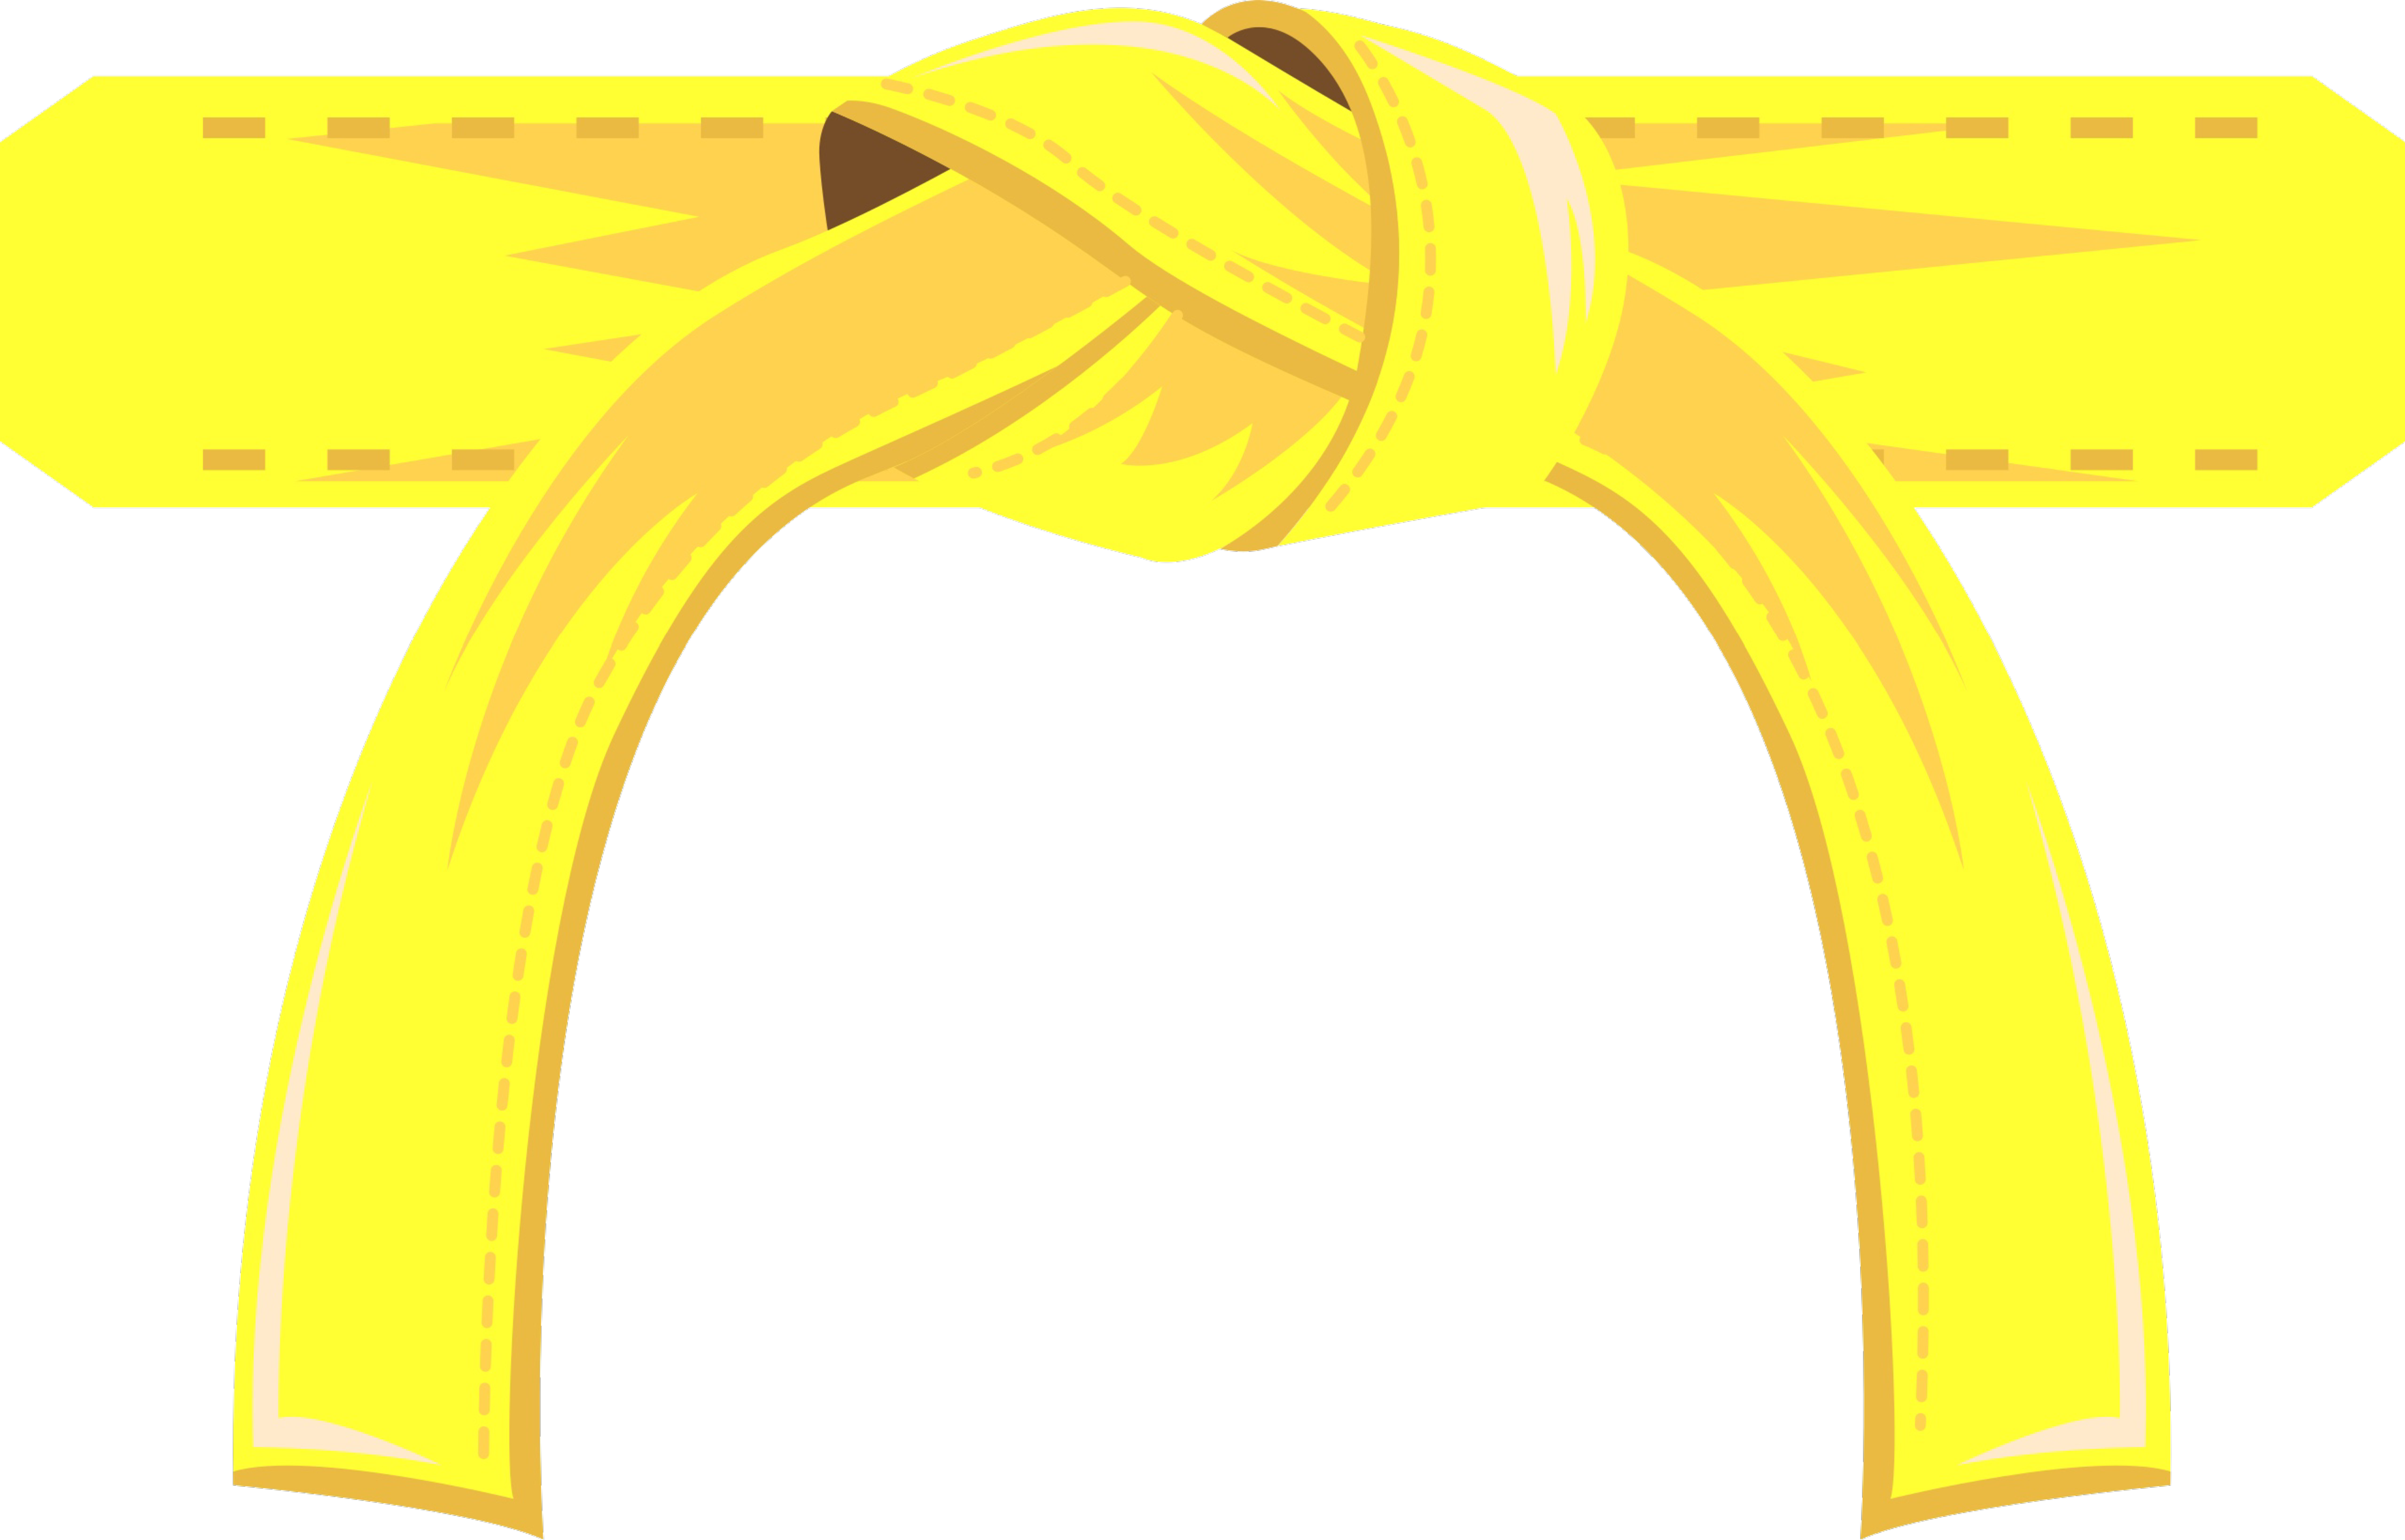
\includegraphics[height=24pt]{Gfx/gurte/yellowbelt}}\\&\\ \text{7.\,Ky\={u}}& \raisebox{-7.2pt}{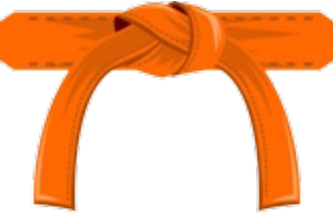
\includegraphics[height=24pt]{Gfx/gurte/orangebelt}}\end{array} \right\}\text{Unterstufe}$\quad$\left.\begin{array}{cl} \text{6.\,Ky\={u}} & \raisebox{-7.2pt}{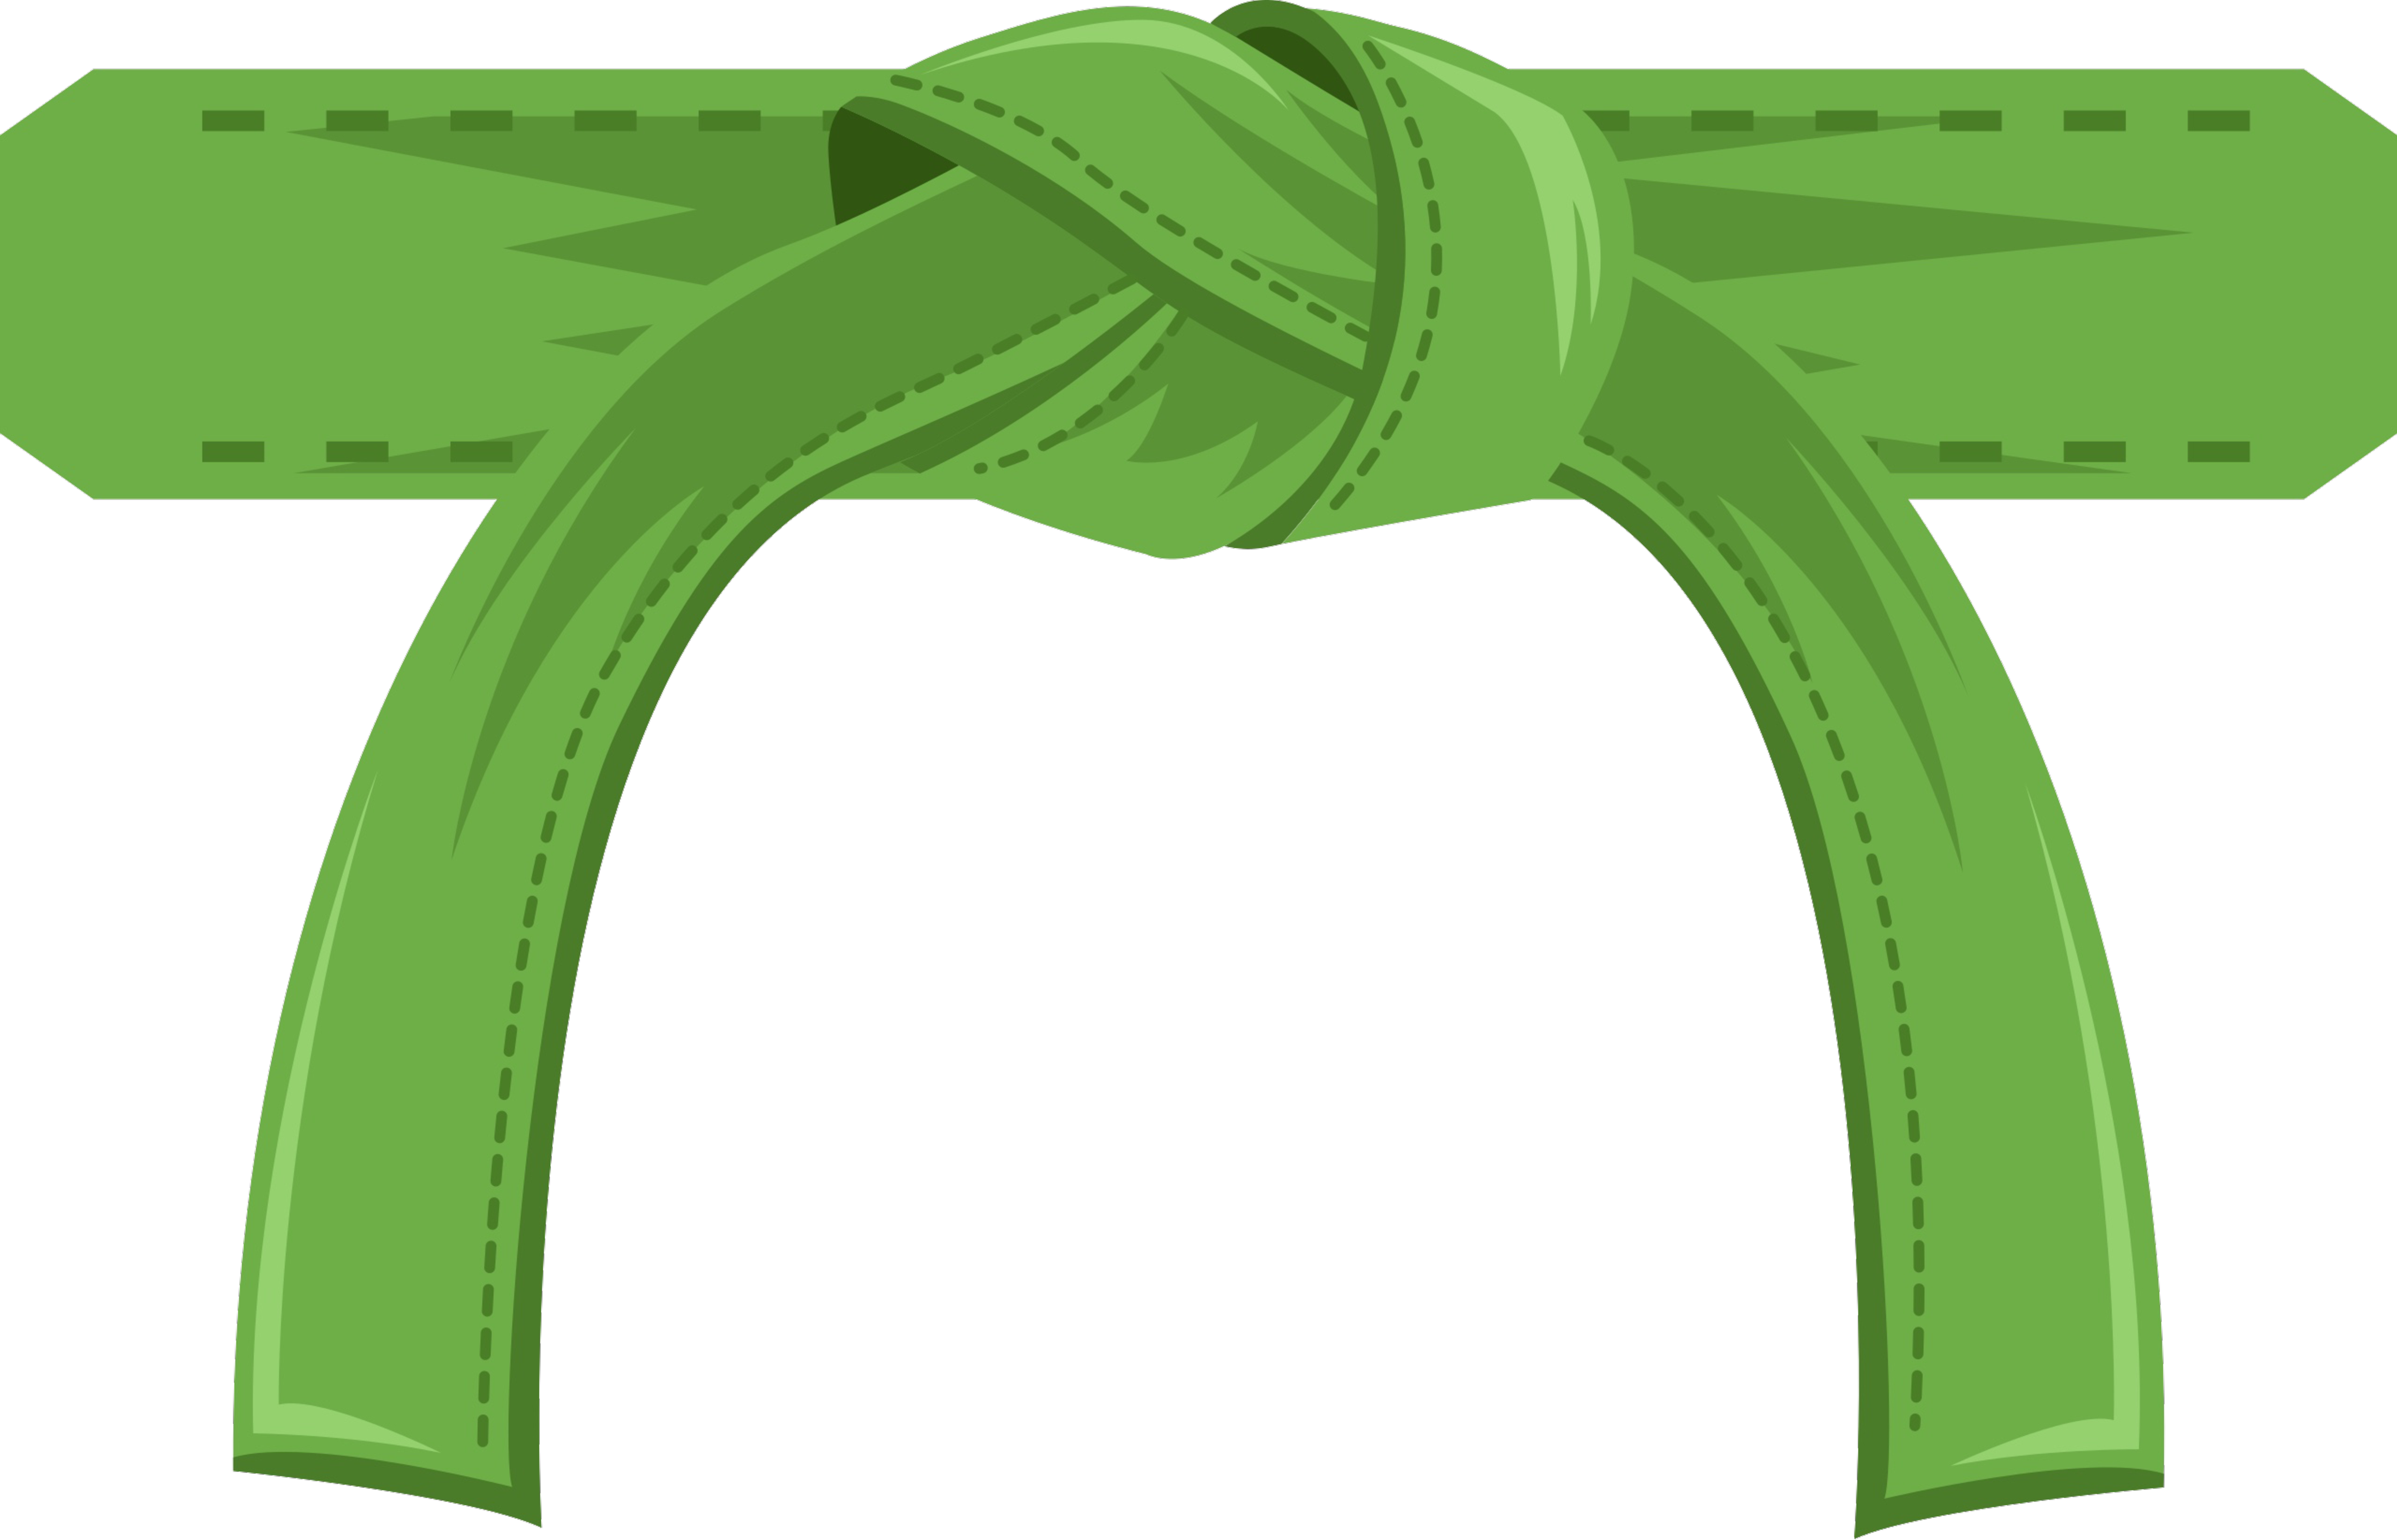
\includegraphics[height=24pt]{Gfx/gurte/greenbelt}}\\&\\ \text{5.\,Ky\={u}} & \raisebox{-7.2pt}{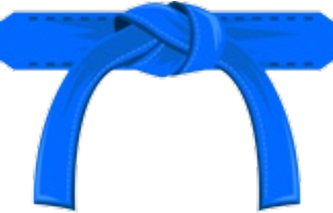
\includegraphics[height=24pt]{Gfx/gurte/bluebelt}}\\&\\ \text{4.\,Ky\={u}} & \raisebox{-7.2pt}{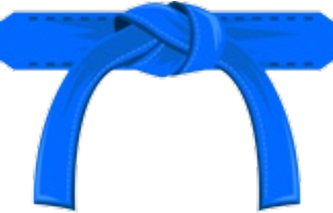
\includegraphics[height=24pt]{Gfx/gurte/bluebelt}}\end{array} \right\}\text{Mittelstufe}$\quad$\left.\begin{array}{cl} \text{3.\,Kyu} & \raisebox{-7.2pt}{
\includegraphics[height=24pt]{Gfx/gurte/brownbelt}}\\&\\ \text{2.\,Ky\={u}} & \raisebox{-7.2pt}{
\includegraphics[height=24pt]{Gfx/gurte/brownbelt}}\\&\\ \text{1.\,Ky\={u}} & \raisebox{-7.2pt}{
\includegraphics[height=24pt]{Gfx/gurte/brownbelt}}\end{array} \right\}\text{Oberstufe}$
		\end{center}		
		Die Ky\={u}grade werden in unserem Dojo von unseren Trainern geprüft. Das jeweilige Prüfungsprogramm, sprich die zugrunde liegenden Techniken, Partnerformen, Kata sowie Kata-Bunkai, sind auf entsprechenden Trainingskarten beschrieben. \textit{\underline{Anmerkun}}g: zum 4.\,Ky\={u} wird bei uns \textit{nicht} auf einen \textit{violetten} Gürtel gewechselt, wir \textit{bleiben} auf \textit{blau}.\\		
		\textit{Besonderheiten:} Der Prüfungsinhalt zum 1.\,Kyu umfasst, zusätzlich zum eigentlichen Programm, ebenfalls die Inhalte der ebenfalls an diesem Tag stattfindenden Prüfungen - wenn zum Beispiel zur Prüfung zum 1.\,Kyu zwei Karateka angemeldet sind, sowie jeweils ein Karateka zum 9.,\,5.\,und 7.\,Kyu, so gehen die beiden zuerst genannten die jeweiligen Prüfungsprogramme der anderen ebenfalls mit, mit Ausnahme von Partnerformen und Kata-Bunkai. Findet an diesem Tag keine andere Prüfung statt, werden weitere Prüfinhalte im Vorfeld abgesprochen.}
	\end{center}\null\vfill\null
	\setlength{\tabcolsep}{6pt}
\end{tcolorbox}
%%------------------------------------------------------------------------------
\pagebreak
%%------------------------------------------------------------------------------
%%Kyu_2
%%------------------------------------------------------------------------------
\begin{tcolorbox}[colback=white,colframe=GKD,coltitle=white,adjusted title=Entwicklungsweg entlang der Kyu-Grade]
	\null\vfill\null
	\begin{tabularx}{\linewidth}{XXX}
		9.-7. Ky\={u}	& 6.-4. Ky\={u}	& 3.-1. Ky\={u}\\
		\midrule
		{\footnotesize \textbf{Kihon}}&{\footnotesize \textbf{Kihon}}&{\footnotesize \textbf{Kihon}}\\
		{\footnotesize Erste Schwerpunkte sind individuell korrekte Dachi-Waza, die aufrechte Haltung des Oberkörpers und die Synchronität von Körperbewegung, Stellung und Technik. Die Prüflinge zum 7. Ky\={u} sollten bereits gute Ansätze innerer und äußerer Spannung zeigen.}&{\footnotesize Die Techniken sollten bereits flüssig sein und Kime sollte bereits deutlich erkennbar sein. Kombinationen dürfen weder hastig in der Ausführung sein, noch überlaufen werden, sondern müssen als Kombination der Einzeltechniken sichtbar sein.}&{\footnotesize Kime, Geschwindigkeit und Körperspannung sind eindeutig vorhanden. Jede Technik aus dem bis hierhin geforderten Kihon wird beherrscht, sowohl als Einzeltechnik, als auch in Kombination.}\\
		{\footnotesize \textbf{Kata}}&{\footnotesize \textbf{Kata}}&{\footnotesize \textbf{Kata}}\\
		{\footnotesize Hoch- und Tief-Bewegungen sollten bereits vermieden werden und die Spannung im Endpunkt sollte bereits erkennbar dargestellt werden. Ab dem 7. Ky\={u} auf sollte bereits auf Rhythmus, sowie Spannung/Entspannung geachtet werden.}&{\footnotesize Ablauf und Kime der Kata sind bereits stimmig und an den dynamischen Stellen der Kata ist die Ernsthaftigkeit deutlich erkennbar. Kiai wird deutlich, konsequent und richtig gesetzt, die jeweilige Technik wird mit deutlichem Kime ausgeführt.}&{\footnotesize Die zu prüfende Kata des jeweiligen Grades sollte die Arbeit aus dem Training widerspiegeln. Die Ernsthaftigkeit ist bis zum Ende aufrechtzuerhalten und immer klar erkennbar. Kata ist auch Kampf, dieses sollte klar gezeigt werden.}\\
		{\footnotesize \textbf{Partnerformen}}&{\footnotesize \textbf{Partnerformen \& Bunkai}}&{\footnotesize \textbf{Partnerformen, Bunkai \& SV}}\\
		{\footnotesize Kihon-Ippon Kumite Formen sollten wechselseitig, bei steigender Graduierung mit wachsender Ernsthaftigkeit gezeigt werden. Distanzen werden korrekt eingenommen.}&{\footnotesize Kumite-Ura und Nage-Waza werden in korrektem Ablauf, optimaler Distanz und graduierungsgerechter Intensität gezeigt. Bunkai wird schulmäßig vorgeführt.}&{\footnotesize Bunkai wird bereits intensiv gezeigt und gekämpft, in schulmäßiger Form. Auf \mbox{Okuden} und \mbox{Renzoku} wird verzichtet, lediglich \mbox{Omote} Techniken werden gezeigt. Die SV wird realitätsnah, aber nicht übertrieben, gezeigt.}
	\end{tabularx}\null\vfill\null
\end{tcolorbox}
%%------------------------------------------------------------------------------
\pagebreak
%%------------------------------------------------------------------------------
%%Waffen_1
%%------------------------------------------------------------------------------
\begin{tcolorbox}[colback=white,colframe=GKD,coltitle=white,adjusted title=Waffen]
	\null\vfill\null	
	\begin{tabularx}{\linewidth}{cccc}
		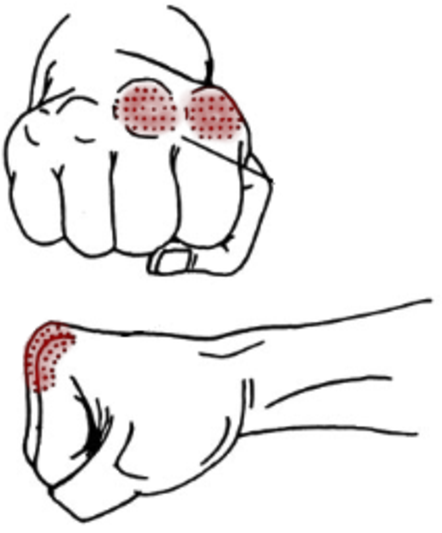
\includegraphics[height=0.119\textwidth-2\tabcolsep,keepaspectratio]{Gfx/habersetzer/habersetzer_waffen_hand_seiken}	& 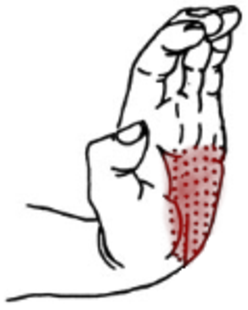
\includegraphics[height=0.119\textwidth-2\tabcolsep,keepaspectratio]{Gfx/habersetzer/habersetzer_waffen_hand_teisho}	& 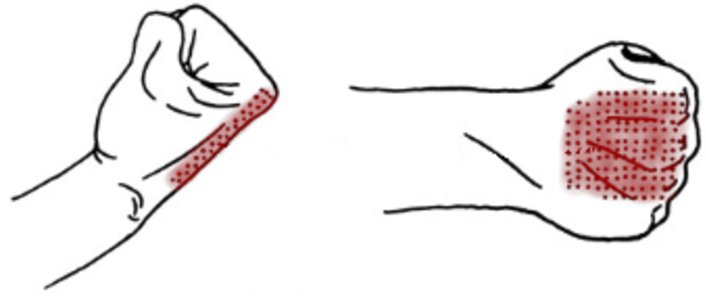
\includegraphics[height=0.119\textwidth-2\tabcolsep,keepaspectratio]{Gfx/habersetzer/habersetzer_waffen_hand_uraken}	& 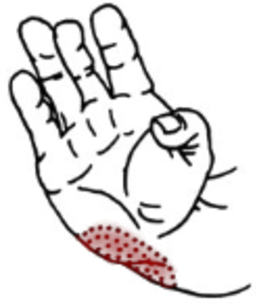
\includegraphics[height=0.119\textwidth-2\tabcolsep,keepaspectratio]{Gfx/habersetzer/habersetzer_waffen_hand_seiryuto} \\
		Seiken 	& Teish\={o} 	& Uraken 	& Seiry\={u}t\={o}\\&&&\\
		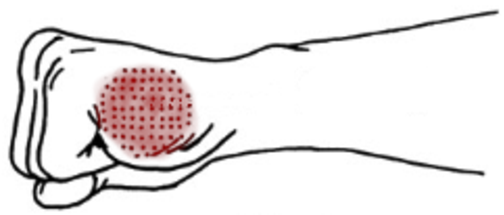
\includegraphics[height=0.119\textwidth-2\tabcolsep,keepaspectratio]{Gfx/habersetzer/habersetzer_waffen_hand_tettsui} & 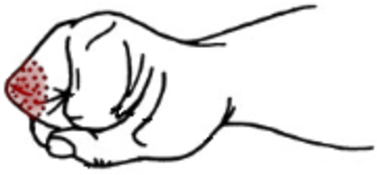
\includegraphics[height=0.119\textwidth-2\tabcolsep,keepaspectratio]{Gfx/habersetzer/habersetzer_waffen_hand_nakadaka_ippon_ken} & 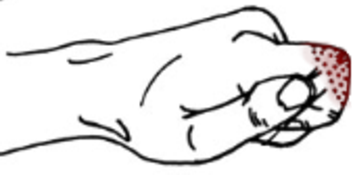
\includegraphics[height=0.119\textwidth-2\tabcolsep,keepaspectratio]{Gfx/habersetzer/habersetzer_waffen_hand_ippon_ken} & 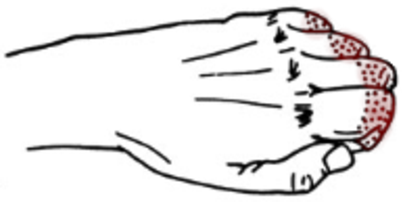
\includegraphics[height=0.119\textwidth-2\tabcolsep,keepaspectratio]{Gfx/habersetzer/habersetzer_waffen_hand_hiraken} \\
		Tettsui 	& Nakadaka 	& Ippon Ken & Hiraken \\&&&\\
		
\includegraphics[height=0.119\textwidth-2\tabcolsep,keepaspectratio]{Gfx/habersetzer/habersetzer_waffen_hand_haito} & 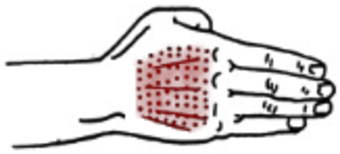
\includegraphics[height=0.119\textwidth-2\tabcolsep,keepaspectratio]{Gfx/habersetzer/habersetzer_waffen_hand_haishu}	& 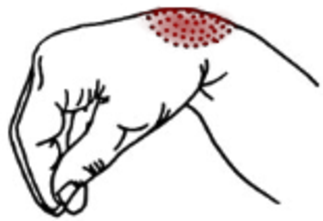
\includegraphics[height=0.119\textwidth-2\tabcolsep,keepaspectratio]{Gfx/habersetzer/habersetzer_waffen_hand_koken} & 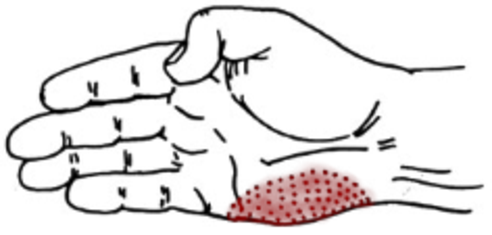
\includegraphics[height=0.119\textwidth-2\tabcolsep,keepaspectratio]{Gfx/habersetzer/habersetzer_waffen_hand_shuto} \\
		Hait\={o} 	& Haishu 	& Koken 		& Shut\={o} \\&&&\\	
		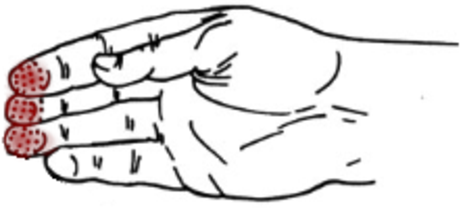
\includegraphics[height=0.119\textwidth-2\tabcolsep,keepaspectratio]{Gfx/habersetzer/habersetzer_waffen_hand_nukite}	& 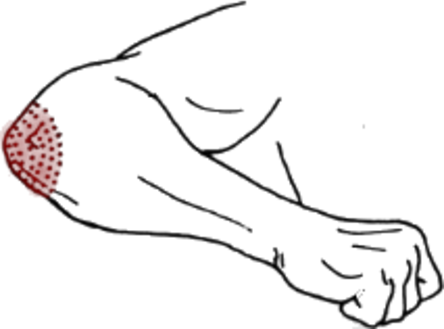
\includegraphics[height=0.119\textwidth-2\tabcolsep,keepaspectratio]{Gfx/habersetzer/habersetzer_waffen_hand_empi} &  & \\
		Nukite 	& Empi 		&  			& \\
	\end{tabularx}
	\null\vfill\null
\end{tcolorbox}
%%------------------------------------------------------------------------------
\pagebreak
%%------------------------------------------------------------------------------
%%Waffen_2
%%------------------------------------------------------------------------------
\begin{tcolorbox}[colback=white,colframe=GKD,coltitle=white,adjusted title=Waffen]
	\null\vfill\null	
	\begin{tabularx}{\textwidth}{cccc}
		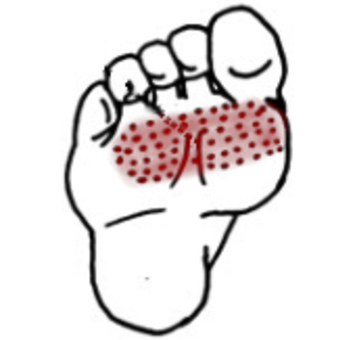
\includegraphics[height=0.18\textwidth-2\tabcolsep,keepaspectratio]{Gfx/habersetzer/habersetzer_waffen_fuss_koshi} 		& 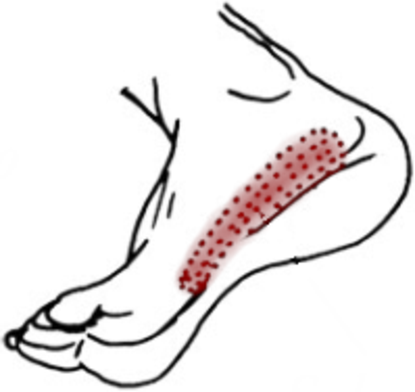
\includegraphics[height=0.18\textwidth-2\tabcolsep,keepaspectratio]{Gfx/habersetzer/habersetzer_waffen_fuss_sokuto} 		& 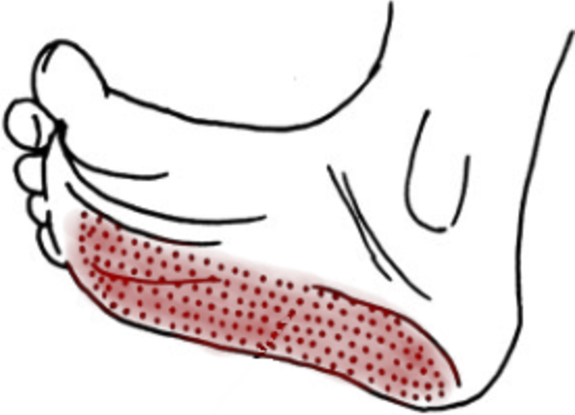
\includegraphics[height=0.18\textwidth-2\tabcolsep,keepaspectratio]{Gfx/habersetzer/habersetzer_waffen_fuss_teisoku} &
		\multirow{3}{*}{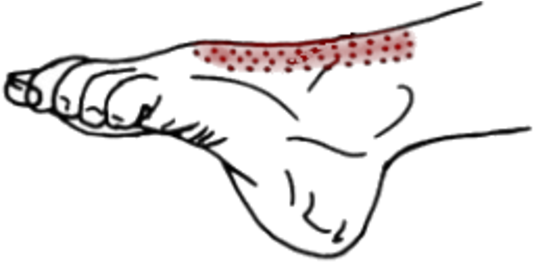
\includegraphics[height=0.18\textwidth-2\tabcolsep,keepaspectratio]{Gfx/habersetzer/habersetzer_waffen_fuss_haisoku}}\\
		Ch\={u}soku 		& Sokut\={o} 	& Teisoku &\\&&&\\&&&\\&&&\\
		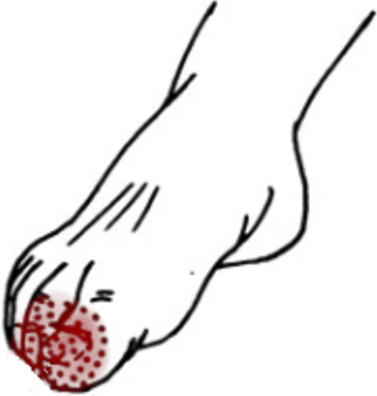
\includegraphics[height=0.18\textwidth-2\tabcolsep,keepaspectratio]{Gfx/habersetzer/habersetzer_waffen_fuss_tsumasaki} 	& 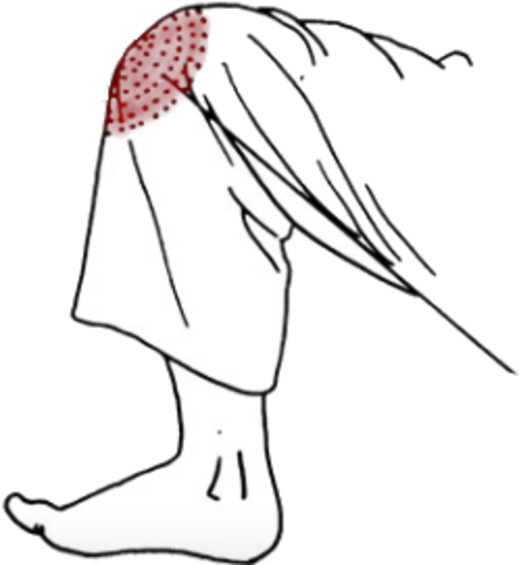
\includegraphics[height=0.18\textwidth-2\tabcolsep,keepaspectratio]{Gfx/habersetzer/habersetzer_waffen_fuss_hiza} 		&  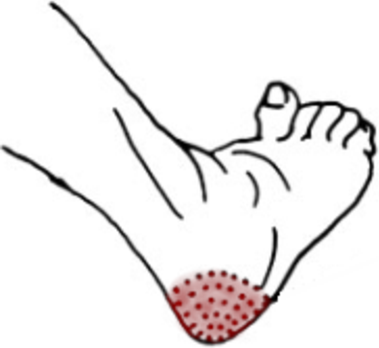
\includegraphics[height=0.18\textwidth-2\tabcolsep,keepaspectratio]{Gfx/habersetzer/habersetzer_waffen_fuss_kakato} &\\
		Tsumasaki 	& Hiza 		& Kakato & Haisoku\\
	\end{tabularx}
	\null\vfill\null
\end{tcolorbox}
%%------------------------------------------------------------------------------
\pagebreak
%%------------------------------------------------------------------------------
%%Dachi
%%------------------------------------------------------------------------------
\begin{tcolorbox}[colback=white,colframe=GKD,coltitle=white,adjusted title=Hinweise zu Dachi-Waza]
	\null\vfill\null
	\begin{tabularx}{\textwidth}{cccc}
		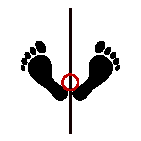
\includegraphics[width=0.25\textwidth-2\tabcolsep,keepaspectratio]{Gfx/self/musubi_dachi.pdf}	&
		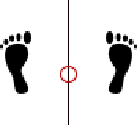
\includegraphics[width=0.25\textwidth-2\tabcolsep,keepaspectratio]{Gfx/self/heiko_dachi.pdf} &
		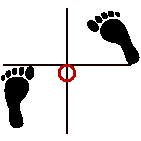
\includegraphics[width=0.25\textwidth-2\tabcolsep,keepaspectratio]{Gfx/self/sanchin_dachi.pdf} & \\
		Musubi Dachi 		& Heik\={o} Dachi 	& Sanchin Dachi & \\
		
\includegraphics[width=0.25\textwidth-2\tabcolsep,keepaspectratio]{Gfx/self/nekoashi_dachi.pdf} & \multicolumn{2}{c}{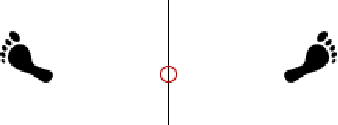
\includegraphics[width=0.5\textwidth-1\tabcolsep,keepaspectratio]{Gfx/self/shiko_dachi.pdf}} & \multirow[t]{3}{*}{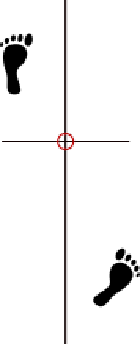
\includegraphics[width=0.25\textwidth-2\tabcolsep,keepaspectratio]{Gfx/self/zenkutsu_dachi.pdf}}\\
		Neko-Ashi Dachi 	& \multicolumn{2}{c}{Shiko Dachi} 	& Zenkutsu Dachi  \\							
	\end{tabularx}\\\null\vfill\null
\end{tcolorbox}
%%------------------------------------------------------------------------------
\pagebreak
%%------------------------------------------------------------------------------
%%Kata_Kyu_Dan
%%------------------------------------------------------------------------------
\begin{tcolorbox}[colback=white,colframe=GKD,coltitle=white,adjusted title=Kata des G\={o}j\={u}-Ry\={u} Karate-D\={o}]
	\null\vfill\null
	\begin{tabularx}{\linewidth}{XXX}
		\textbf{Taikyoku-Kata}	& \textbf{Kata im Ky\={u}-Bereich}	& \textbf{Kata im Dan-Bereich}\\
		\midrule
		{\small Taikyoku J\={o}dan}		&{\small Gekisai-Dai-Ichi\textsuperscript{1}}	&{\small Shis\={o}chin\textsuperscript{1}}\\
		{\small Taikyoku Ch\={u}dan}	&{\small Gekisai-Dai-Ni\textsuperscript{1}}	&{\small Seisan\textsuperscript{1}}\\
		{\small Taikyoku Gedan}			&{\small Saif\={a}\textsuperscript{1}}			&{\small S\={e}pai\textsuperscript{1}}\\
		{\small Taikyoku Kake-Uke}		&{\small S\={e}enchin\textsuperscript{1}}		&{\small Kururunf\={a}\textsuperscript{1}}\\
		{\small Taikyoku Joshugi}		&{\small Tensh\={o}\textsuperscript{2}}		&{\small S\={u}p\={a}rinpei\textsuperscript{1}} \textit{(Petch\={u}rin)}\\
		{\small Taikyoku Mawashi-Uke}	&{\small Sanchin\textsuperscript{2}}			&\\
										&{\small Sans\={e}ru\textsuperscript{1}}		&\\
	\end{tabularx}\\
	{\small	
	\begin{description}
		\item[Taikyoku Katas] Die Taikyoku Katas haben alle das identische Enbusen gemeinsam, sie unterscheiden sich lediglich in der jeweiligen Blocktechnik sowie der Konteraktion. Sie werden auch Fukyu-Kata (">verbreitete"< oder Anfänger-Kata) genannt.
		\begin{description}
			\item[J\={o}dan] \tabto{50pt}Age-Uke\bull Oi-Zuki J\={o}dan
			\item[Ch\={u}dan] \tabto{50pt}Yoko-Uke\bull Oi-Zuki Ch\={u}dan
			\item[Gedan] \tabto{50pt}Harai-Otoshi-Uke\bull Oi-Zuki Gedan
			\item[Kake-Uke]\tabto{50pt}Kake-Uke\bull Mae-Geri Ch\={u}dan\bull Hiji-Ate
			\item[Mawashi-Uke] \tabto{50pt}Mawashi-Uke\bull Mawashi-Empi-Uke\bull Uraken-Uchi\bull Harai-Otoshi-Uke\bull Gyaku-Zuki Ch\={u}dan
			\item[Joshugi] \tabto{50pt}Kombination aus J\={o}dan, Ch\={u}dan und Gedan
		\end{description}
	\end{description}\bigskip\rule{141pt}{.4pt}\\
	{\footnotesize
	\textsuperscript{1} Kaishu Kata - häufig als Kata der offenen Hand übersetzt, beschreibt aber den Spannungszustand in der Bewegung ">locker"<\\
	\textsuperscript{2} Haishu Kata - häufig als Kata der geschlossenen Hand übersetzt, beschreibt aber den Spannungszustand in der Bewegung ">angespannt"<}
	}\null\vfill\null
\end{tcolorbox}
%%------------------------------------------------------------------------------
\pagebreak
%%------------------------------------------------------------------------------
%%Basiskombinationen
%%------------------------------------------------------------------------------
\begin{tcolorbox}[colback=white,colframe=GKD,coltitle=white,adjusted title=Basiskombination]
	\setlength{\tabcolsep}{3pt}		
	\null\vfill\null
	\begin{tabularx}{\textwidth}{llXXX}
		\textbf{Stand} 		& & \textbf{Technik 1\,\(\odot\)} 	& \textbf{Technik 2\,\(\odot\)} 	& \textbf{Technik 3\,\(\odot\)}\\
		\midrule
		Sanchin Dachi 		& \(\hookleftarrow\)	& Age-Uke				& Kake-Uke 				& Harai-Otoshi-Uke	\\
		\textit{oder}		& \(\hookrightarrow\) 	& Zuki J\={o}dan 		& Teish\={o}-Zuki Gedan		& Ura-Zuki			\\
		Zenkutsu Dachi		& \(\hookleftarrow\)	& Yoko-Uke 				& Shut\={o}-Uke 			& Gedan Teish\={o}-Uke	\\
		\textit{oder}		& \(\hookrightarrow\)	& Zuki Ch\={u}dan 		& Nukite (Kehle) 		& Uraken-Uchi		\\
		Shiko Dachi			& \(\hookleftarrow\)	& Soto-Uke 				& Mawashi-Uke 			& Haishu-Uke		\\
		& \(\hookrightarrow\)	& Ch\={u}dan-Zuki	& Teish\={o}-Ate 		& Furi-Uchi			\\
		\midrule
		\textbf{Stand} 		& & \textbf{Technik\,\(\odot\)} 		&  						&\\
		\midrule
		Sanchin Dachi 		& \(\hookrightarrow\)	& Oi-Zuki J\={o}dan 	&  						&\\
		Zenkutsu Dachi		& \(\hookrightarrow\)	& Oi-Zuki Ch\={u}dan 	&\multicolumn{2}{l}{Nach Abschluss dann}\\
		Shiko Dachi			& \(\hookrightarrow\)	& Oi-Zuki Gedan 		&\multicolumn{2}{l}{seitengedreht von oben weiter}\\
		Shiko Dachi			& \(\hookleftarrow\)	& Harai-Otoshi-Uke 		&  						&\\
		Zenkutsu Dachi		& \(\hookleftarrow\)	& Yoko-Uke 				&  						&\\
		Sanchin Dachi		& \(\hookleftarrow\)	& Age-Uke 				&  						&\\
	\end{tabularx}\\\null\vfill\null
	\setlength{\tabcolsep}{6pt}	
	\begin{center}
		\parbox{\textwidth-\tabcolsep}{Koordinationsübungen im Kihon. Im oberen Block  können Stände und Techniken beliebig gemischt werden. Der untere Block ist zur Übung der Fußbewegungen in der Vorwärts-, bzw. Rückwärtsbewegung gedacht.}
	\end{center}
	\null\vfill\null
\end{tcolorbox}
%%------------------------------------------------------------------------------
\pagebreak
%%------------------------------------------------------------------------------
%%Zuki_Kata
%%------------------------------------------------------------------------------
\begin{tcolorbox}[colback=white,colframe=GKD,coltitle=white,adjusted title=Zuki Kata aus dem Japan Karate-D\={o} Jinen-Kai]
	\null\vfill\null
	\begin{center}
		\parbox{\textwidth-2\tabcolsep}{Basiskombination für Zuki im Zenkutsu-Dachi. Diese Kombination dient der Übung der Suri-Ashi (gleitende Schritte) im Zenkutsu-Dachi. Nach Abschluss der ersten Sequenz über Mawatte einen Seiten-/Richtungswechsel vornehmen und den Rückweg gehen.}
	\end{center}
	\begin{tabularx}{\textwidth}{lllX}
		%\multicolumn{7}{l}{\textbf{Konishi}}\\
		Stand	&&Technik	&\\
		\midrule
		Zenkutsu Dachi 	& \(\hookleftarrow\) & Harai-Otoshi-Uke	&\\
		Zenkutsu Dachi 	& \(\hookrightarrow\) & Oi-Zuki J\={o}dan	&\\
		Zenkutsu Dachi 	& \(\hookrightarrow\) & Ren-Zuki J\={o}dan \&~Ch\={u}dan	&\\
		Zenkutsu Dachi 	& \(\hookrightarrow\) & Gyaku-Zuki Ch\={u}dan	&2x schnell vorgehen\\
		Zenkutsu Dachi 	& \(\hookrightarrow\) & Gyaku-Zuki J\={o}dan	&\\
		Zenkutsu Dachi 	& \(\hookrightarrow\) & Gyaku-Zuki Ch\={u}dan	&2x schnell vorgehen\\
		Zenkutsu Dachi 	& \(\hookrightarrow\) & Harai-Otoshi-Uke	& Mawatte \& seitengespiegelt von oben\\
		\midrule
	\end{tabularx}\\\null\vfill\null
\end{tcolorbox}
%%------------------------------------------------------------------------------
\pagebreak
%%------------------------------------------------------------------------------
%%Bogyo Roku Kyodo
%%------------------------------------------------------------------------------
\begin{tcolorbox}[colback=white,colframe=GKD,coltitle=white,adjusted title=B\={o}gy\={o} R\={o}k\={u} Kyod\={o} aus dem Japan Karate-D\={o} Jinen-Kai]
	\null\vfill\null
	\begin{center}
		\parbox{\textwidth-2\tabcolsep}{Es werden alle 6 Stände \& Techniken am Stück durchgeführt, in der Art, das immer der jeweils vordere Arm blockt (bzw. für die Fußtechniken der vordere Fuß kickt) und alle Standwechsel lediglich über den vorderen Fuß erfolgen. Als erste Übungsform wird nur der Block ausgeführt, als nächste Steigerungsform wird der Konter hinzugenommen, als letzte Steigerung dann \mbox{Block \(\Rightarrow\)\,Kick \(\Rightarrow\)\,Konter.}}
	\end{center}
	\begin{tabularx}{\textwidth}{lllXlXll}
		%\multicolumn{7}{l}{\textbf{Konishi}}\\
		Stand	&&Block	&&Konter	&&Kick&\\
		\midrule
		Zenkutsu Dachi 	& \(\hookrightarrow\) & Age-Uke	&&Gyaku-Zuki	&&Mae-Geri&\textbf{Konishi Form}\\
		Shiko Dachi 	& \(\circledast\) & Harai-Otoshi-Uke	&&Kagi-Zuki&&Yoko-Geri&\\
		Zenkutsu Dachi	& \(\circledast\) & Yoko-Uke	&&Gyaku-Zuki&&Mae-Geri&\\
		Zenkutsu Dachi	& \(\circledast\) & Soto-Uke	&&Gyaku-Zuki&&Mae-Geri&\\
		Neko-Ashi Dachi	& \(\circledast\) & Shut\={o}-Uke	&&Nukite&&Kansetsu-Geri&\\
		Shiko Dachi	& \(\hookleftarrow\) & Hait\={o}-Uke	&&Gyaku-Zuki&&Ashi-Barai& \(\odot\)\\
		\midrule
	\end{tabularx}\\\null\vfill\null
\end{tcolorbox}
%%------------------------------------------------------------------------------
\pagebreak
%%------------------------------------------------------------------------------
%%Kihon Ippon Kumite
%%------------------------------------------------------------------------------
\begin{tcolorbox}[colback=white,colframe=GKD,coltitle=white,adjusted title=Kihon-Ippon-Kumite]
	\null\vfill\null
	{\small 	
		\begin{tabularx}{\textwidth}{llllX}
			\textbf{Stufe} 	& \textbf{Angriff} 	& \textbf{Block}&\textbf{Konter}&Anmerkung\\
			\midrule
			J\={o}dan 	& Oi-Zuki 	& Age-Uke			&Gyaku-Zuki	& Angriff rechts, Block links, Konter rechts Ch\={u}dan \\
			J\={o}dan 	& Oi-Zuki 	& Age-Uke			&Gyaku-Zuki	& Angriff rechts, Block rechts, Konter links Ch\={u}dan \\	
			Ch\={u}dan	& Oi-Zuki	& Yoko-Uke			&Gyaku-Zuki	& Angriff rechts, Block links, Konter rechts Ch\={u}dan \\
			Ch\={u}dan	& Oi-Zuki	& Soto-Uke			&Gyaku-Zuki	& Angriff rechts, Block links, Konter rechts Ch\={u}dan \\
			Ch\={u}dan	& Ura-Zuki	& Soto-Uke			&Gyaku-Zuki	& Angriff rechts, Block links, Konter rechts J\={o}dan \\
			Ch\={u}dan	& Oi-Zuki	& Shut\={o}-Uke		&Gyaku-Zuki	& Angriff rechts, Block links, Konter rechts \\
			Ch\={u}dan	& Oi-Zuki	& Shut\={o}-Uke		&Gyaku-Zuki	& Angriff rechts, Block rechts, Konter links \\
			Gedan		& Oi-Zuki	& Harai-Otoshi-Uke	&Gyaku-Zuki	& Angriff rechts, Block links, Konter rechts  \\
			Gedan		& Mae-Geri	& Harai-Otoshi-Uke	&Gyaku-Zuki	& Angriff rechts, Block links, Konter rechts \\
			Gedan		& Mae-Geri	& Nagashi-Uke		&Gyaku-Zuki	& Angriff rechts, Block links (rechts), Konter rechts (links)\\
			\midrule
		\end{tabularx}
	}\null\vfill\null
	\begin{minipage}[t]{\textwidth}
		{\footnotesize 
			Als grundlegende Partnerformen der Unterstufe sollten die Techniken mit, dem jeweiligen Können entsprechender, Geschwindigkeit und Definition gezeigt werden. Stete Übung bringt Schnelligkeit. Zu beachten sind die richtige Distanz zum Partner und die korrekte Reaktion auf wechselnde Abstände - Kontertechniken mit Kime setzen. Die Basisübungen sind in der Form \textit{Gerader Angriff - Gerader Konter} beschrieben, sollten aber auch in den Sh\={o}t\={o}kan Varianten mit jeweils 45°-Ausweichbewegungen geübt werden, sind aber nicht Prüfungsrelevant. Dann sind kleinere Anpassungen notwendig, bzw.\,möglich, die sich aus dem Übungsansatz ergeben. Kontertechniken können, und dürfen, entsprechend dem jeweiligen Leistungsstand variiert werden.
		}%\onehalfspacing\singlespacing
		{\footnotesize 
			Die Partnerformen können als \textbf{\textit{Drill}} geübt werden, indem Tori 10 Techniken mit Vorwärtsbewegung ausführt. Am Ende dann Wechsel von Tori zu Uke und 10 Techniken in die andere Richtung. Bei der Ausführung als Drill ist der stetige Seitenwechsel zu beachten, sowie das jeweilig \textquotedblleft richtige Hikite ziehen\textquotedblright. Im Drill bietet es sich an, den Stand auf Sanchin-Dachi zu verkürzen, bzw. für \textit{Gedan Oi-Zuki} auf Shiko-Dachi zu verlängern.
		}
	\end{minipage}
	\null\vfill\null	
\end{tcolorbox}
%%------------------------------------------------------------------------------
\pagebreak
%%------------------------------------------------------------------------------
%%------------------------------------------------------------------------------
%%Bogyo Roku Kyodo
%%------------------------------------------------------------------------------
\begin{tcolorbox}[colback=white,colframe=GKD,coltitle=white,adjusted title=B\={o}gy\={o} R\={o}k\={u} Kyod\={o} aus dem Japan Karate-D\={o} Jinen-Kai]
	\null\vfill\null
	\begin{center}
		\parbox{\textwidth-2\tabcolsep}{Es werden alle 6 Stände \& Techniken am Stück durchgeführt, in der Art, das immer der jeweils vordere Arm blockt (bzw. für die Fußtechniken der vordere Fuß kickt) und alle Standwechsel lediglich über den vorderen Fuß erfolgen. Als erste Übungsform wird nur der Block ausgeführt, als nächste Steigerungsform wird der Konter hinzugenommen, als letzte Steigerung dann \mbox{Block \(\Rightarrow\)\,Kick \(\Rightarrow\)\,Konter.}}
	\end{center}
	\begin{tabularx}{\textwidth}{lllXlXll}
		%\multicolumn{7}{l}{\textbf{Konishi}}\\
		Stand	&&Block	&&Konter	&&Kick&\\
		\midrule
		Zenkutsu Dachi 	& \(\hookrightarrow\) & Age-Uke	&&Gyaku-Zuki	&&Mae-Geri&\textbf{Konishi Form}\\
		Shiko Dachi 	& \(\circledast\) & Harai-Otoshi-Uke	&&Kagi-Zuki&&Yoko-Geri&\\
		Zenkutsu Dachi	& \(\circledast\) & Yoko-Uke	&&Gyaku-Zuki&&Mae-Geri&\\
		Zenkutsu Dachi	& \(\circledast\) & Soto-Uke	&&Gyaku-Zuki&&Mae-Geri&\\
		Neko-Ashi Dachi	& \(\circledast\) & Shut\={o}-Uke	&&Nukite&&Kansetsu-Geri&\\
		Shiko Dachi	& \(\hookleftarrow\) & Hait\={o}-Uke	&&Gyaku-Zuki&&Ashi-Barai& \(\odot\)\\
		\midrule
	\end{tabularx}\\\null\vfill\null
\end{tcolorbox}
%%------------------------------------------------------------------------------
\pagebreak
%%------------------------------------------------------------------------------
%%Kumite-Ura 1
%%------------------------------------------------------------------------------
\begin{tcolorbox}[colback=white,colframe=GKD,coltitle=white,adjusted title=Kurzbeschreibung Kumite-Ura 1..6]
	\null\vfill\null	
	{\small 	
		\begin{tabularx}{\textwidth}{lllllX}
			\multicolumn{3}{l}{\textbf{1. Form}}&\multicolumn{3}{l}{\textbf{2. Form}}\\
			\midrule
			&Tori:	& Oi-Zuki Ch\={u}dan						&&Tori:	& Oi-Zuki Ch\={u}dan\\
			&Uke:	& Ausweichen ca. 45° Grad links				&&Uke:	& Ausweichen ca. 45° Grad links und Yoko-Uke\\
			&		& \textbf{Konter} Chisai-no-Mawashi-Geri	&&		& \textbf{Konter} Ura-Zuki (kurze Rippe)\\
			&Tori:	& Teish\={o}-Uke (links)						&&Tori:	& Empi-Uke (links)\\
			&		& \textbf{Konter} Ura-Zuki J\={o}dan		&&		& \textbf{Konter} Ura-Zuki J\={o}dan\\
			\midrule&&&&&\\
			\multicolumn{3}{l}{\textbf{3. Form}}&\multicolumn{3}{l}{\textbf{4. Form}}\\
			\midrule
			&Tori:	& 2x Oi-Zuki Ch\={u}dan						&&Tori:	& Oi-Zuki Ch\={u}dan\\
			&Uke:	& gleiten und zurückgehen mit 2xYoko-Uke	&&Uke:	& Drehung 90° Grad links und Nagashi-Uke (">\textit{Saifa}"<)\\
			&		& \textbf{Konter} Mae-Geri oder Hiza-Geri	&&		& \textbf{Konter} Uraken-Uchi J\={o}dan\\
			&Tori:	& Teish\={o}-Uke (links)						&&Tori:	& Arme zur Deckung hoch (ähnlich J\={u}ji-Uke)\\
			&		& \textbf{Konter} Ura-Zuki J\={o}dan		&&		& \textbf{Konter} Kansetsu-Geri und Tettsui-Uchi\\
			\midrule&&&&&\\
			\multicolumn{3}{l}{\textbf{5. Form}}&\multicolumn{3}{l}{\textbf{6. Form}}\\
			\midrule
			&Tori:	& Oi-Zuki Ch\={u}dan						&&Tori:	& Oi-Zuki Ch\={u}dan\\
			&Uke:	& Zurück über Neko-Ashi-Dachi mit Teish\={o}-Uke&&Uke:	& Ausweichen ca. 45° Grad links und Teish\={o}-Uchi\\
			&		& \textbf{Konter} Suri-Ashi vorgehen mit Uraken-Uchi	
																&&		& \textbf{Konter} Furi-Uchi-Ken J\={o}dan\\
			&Tori:	& Age-Uke (links)							&&Tori:	& \={O}-Age-Uke\\
			&		& \textbf{Konter} Ura-Zuki J\={o}dan		&&		& \textbf{Konter} Ura-Zuki J\={o}dan\\
			\midrule
		\end{tabularx}
	}\null\vfill\null
\end{tcolorbox}
%%------------------------------------------------------------------------------
\pagebreak
%%------------------------------------------------------------------------------
%%Kumite-Ura 2
%%------------------------------------------------------------------------------
\begin{tcolorbox}[colback=white,colframe=GKD,coltitle=white,adjusted title=Kurzbeschreibung Kumite-Ura 7..12]
	\null\vfill\null	
	{\small 	
		\begin{tabularx}{\textwidth}{lllllX}
			\multicolumn{3}{l}{\textbf{7. Form}}&\multicolumn{3}{l}{\textbf{8. Form ">einarmiger Bandit"<}}\\
			\midrule
			&Tori:	& Oi-Zuki Ch\={u}dan						&&Tori:	& Oi-Zuki Ch\={u}dan\\
			&Uke:	& Ausweichen ca. 45° Grad mit Teish\={o}-Uke links
																&&Uke:	& Links zurück Sanchin-Dachi Osae-Uke\\
			&		& \textbf{Konter} Ura-Zuki J\={o}dan		&&		& \textbf{Konter} Sanchin-Dachi J\={o}dan Teish\={o}-Zukii\\
			&Tori:	& J\={o}dan Teish\={o}-Uke (links)				&&Tori:	& Yoko-Uke (links)\\
			&		& \textbf{Konter} Zenkutsu-Dachi Kagi-Zuki	&&		& \textbf{Konter} Ura-Zuki J\={o}dan\\
			\midrule&&&&&\\
			\multicolumn{3}{l}{\textbf{9. Form}}&\multicolumn{3}{l}{\textbf{10. Form}}\\
			\midrule
			&Tori:	& Oi-Zuki Ch\={u}dan						&&Tori:	& Oi-Zuki Ch\={u}dan\\
			&Uke:	& rechts zurück	und Ura Teish\={o}-Uke			&&Uke:	& Yoko-Uke mit Tsukame \\
			&		& \textbf{Konter} Mae-Geri unter linke Achsel
																&&		& \textbf{Konter} Shiko-Dachi 90° links Shut\={o}-Uchi\\
			&Tori:	& Otoshi-Empi-Uke							&&Tori:	& Shiko-Dachi 90° links Age-Uke rechts\\
			&		& \textbf{Konter} Ura-Zuki/Gyaku-Zuki J\={o}dan	rechts/links
																&&		& \textbf{Konter} Gedan Ura-Zuki links\\
			\midrule&&&&&\\
			\multicolumn{3}{l}{\textbf{11. Form}}&\multicolumn{3}{l}{\textbf{12. Form}}\\
			\midrule
			&Tori:	& Oi-Zuki Ch\={u}dan						&&Tori:	& Oi-Zuki Ch\={u}dan\\
			&Uke:	& Zurück Yoko-Uke mit Tsukame				&&Uke:	& Ausweichen ca. 90° Grad rechts\\
			&		& \textbf{Konter} Shiko-Dachi 90° links Ch\={u}dan Empi-Uchi
																&&		& \textbf{Konter} Teish\={o}-Zuki J\={o}dan\\
			&Tori:	& Shiko-Dachi 90° rechts					&&Tori:	& Teish\={o}-Uke\\
			&		& \textbf{Konter} Empi-Uchi Ch\={u}dan		&&		& \textbf{Konter} rechts mit dem Kopf ">abkippen"<, dann Hebel oder Shut\={o}-/Hait\={o}-/Haishu-Uchi\\
			\midrule
		\end{tabularx}
	}\null\vfill\null
\end{tcolorbox}
%%------------------------------------------------------------------------------
\pagebreak
%%------------------------------------------------------------------------------
%%SV_Ideen_1
%%------------------------------------------------------------------------------
 
%\pagebreak
%\begin{tcolorbox}[colback=white,colframe=GKD,coltitle=white,adjusted title=Kihon-Ippon-Kumite]
%	
%\end{tcolorbox}
%%------------------------------------------------------------------------------
\end{document}
%%------------------------------------------------------------------------------
%%EOF
%%------------------------------------------------------------------------------